% =====================================================================
%  Follow the Workers: What LLM Research Agents Can and Cannot Do
%  on a Weak Signal
%  MFE 230GA Final Project, Fall 2026
%
%  Compiler: pdfLaTeX, then BibTeX (Overleaf default).
%  Needs the folders figures/, tables/ and code/ from the repository's report/.
% =====================================================================

\documentclass[11pt,letterpaper]{article}

% ---------------------------------------------------------------------
% 0. Draft switch
% ---------------------------------------------------------------------
\newif\ifdraft
\draftfalse  % \drafttrue shows placeholders (none left)

\usepackage{float}
\usepackage{tikz}
\usetikzlibrary{positioning,arrows.meta,fit,backgrounds,calc}
\usepackage{listings}
\lstset{basicstyle=\footnotesize\ttfamily,breaklines=true,columns=fullflexible,
  frame=leftline,rulecolor=\color{inkgray},xleftmargin=1em,showstringspaces=false}
\newcommand{\fit}[1]{\resizebox{\ifdim\width>\linewidth\linewidth\else\width\fi}{!}{#1}}
\newcommand{\tagc}{{\footnotesize\itshape confirmatory}}
\newcommand{\tagp}{{\footnotesize\itshape post hoc}}
\newcommand{\tagf}{{\footnotesize\itshape forward test}}




% ---------------------------------------------------------------------
% 1. Page and fonts: working-paper conventions (NBER / SSRN style)
% ---------------------------------------------------------------------
\usepackage[hmargin=0.85in,vmargin=0.9in]{geometry}
\usepackage[T1]{fontenc}
\usepackage[utf8]{inputenc}
\IfFileExists{newtxtext.sty}
  {\usepackage{newtxtext}\usepackage{newtxmath}}   % Times (Overleaf)
  {\usepackage{mathptmx}}                          % local fallback
\IfFileExists{inconsolata.sty}
  {\usepackage[scaled=0.92]{inconsolata}}{}        % monospace for prompts and code
\usepackage{microtype}
\linespread{1.08}
\setlength{\parindent}{1.5em}
\setlength{\parskip}{0pt}

% ---------------------------------------------------------------------
% 2. Colour: black text; one dark navy accent for links only.
%    \accenttrue also colours section titles navy (off by default).
% ---------------------------------------------------------------------
\usepackage{xcolor}
\definecolor{navy}{HTML}{003262}      % Berkeley Blue
\definecolor{inkgray}{HTML}{555555}
\newif\ifaccent
\accentfalse
\newcommand{\headcolor}{\ifaccent\color{navy}\fi}

% ---------------------------------------------------------------------
% 3. Maths, tables, figures, lists
% ---------------------------------------------------------------------
\usepackage{amsmath,amssymb}
\usepackage{booktabs,tabularx,threeparttable,multirow}
\usepackage{graphicx}
\usepackage[labelfont=bf,font=small,labelsep=colon,
            justification=justified,singlelinecheck=false]{caption}
\captionsetup[table]{position=top,skip=4pt}
\captionsetup[figure]{position=bottom,skip=6pt}
\usepackage{subcaption}
\usepackage[shortlabels]{enumitem}
\setlist{itemsep=1pt,topsep=3pt,parsep=0pt,leftmargin=1.5em}

% ---------------------------------------------------------------------
% 4. Section headings: plain, black, numbered
% ---------------------------------------------------------------------
\usepackage{titlesec}
\titleformat{\section}
  {\normalfont\large\bfseries\headcolor}{\thesection}{0.7em}{}
\titleformat{\subsection}
  {\normalfont\normalsize\bfseries\headcolor}{\thesubsection}{0.6em}{}
\titleformat{\subsubsection}[runin]
  {\normalfont\normalsize\itshape}{}{0em}{}[.]
\titlespacing*{\section}{0pt}{1.8ex plus .4ex minus .2ex}{0.8ex plus .2ex}
\titlespacing*{\subsection}{0pt}{1.4ex plus .3ex minus .2ex}{0.5ex plus .1ex}
\titlespacing*{\subsubsection}{\parindent}{0.8ex plus .2ex}{0.5em}

% ---------------------------------------------------------------------
% 5. Page style: page number centred at the bottom, no running head
% ---------------------------------------------------------------------
\pagestyle{plain}

% ---------------------------------------------------------------------
% 6. Boxes: no fill, no colour, thin rules only
% ---------------------------------------------------------------------
\usepackage[most]{tcolorbox}

% Protocol and summary panels: rule above and below, like a table
\newtcolorbox{panel}[1]{
  enhanced, breakable, colback=white, boxrule=0pt, frame hidden, sharp corners,
  borderline north={0.5pt}{0pt}{black}, borderline south={0.5pt}{0pt}{black},
  left=0pt, right=0pt, top=4pt, bottom=4pt, before skip=8pt, after skip=8pt,
  title={#1}, fonttitle=\small\bfseries, coltitle=black, colbacktitle=white,
  attach title to upper={\par\smallskip}, fontupper=\small}
\newenvironment{protocolbox}{\begin{panel}{How we kept the test honest}}{\end{panel}}
\newenvironment{answerbox}{\begin{panel}{Summary of findings}}{\end{panel}}

% Prompt box: verbatim text with a thin grey rule on the left
\newtcolorbox{promptbox}[2]{
  enhanced, colback=white, boxrule=0pt, frame hidden, sharp corners,
  borderline west={0.6pt}{0pt}{inkgray},
  left=8pt, right=0pt, top=2pt, bottom=2pt, before skip=6pt, after skip=6pt,
  title={\bfseries #1\hfill\normalfont\itshape #2},
  fonttitle=\small, coltitle=black, colbacktitle=white,
  attach title to upper={\par\smallskip},
  fontupper=\footnotesize\ttfamily\raggedright}

% ---------------------------------------------------------------------
% 7. Macros
% ---------------------------------------------------------------------
\usepackage{xspace}
% Post-hoc marker: a dagger in tables and captions, explained once in 2.3
\newcommand{\ph}{\textsuperscript{\dag}}
\newcommand{\posthocnote}{\dag\,Post hoc: decided after the test period was opened.}
% Names used throughout (Appendix A maps them to the repository)
\newcommand{\StudyOne}{Study~1\xspace}
\newcommand{\StudyOneB}{Study~1b\xspace}
\newcommand{\StudyTwo}{Study~2\xspace}
\newcommand{\HQ}{HQ12\xspace}
% Placeholders and owners (visible in draft only)
\newcommand{\placeholder}[1]{\ifdraft{\color{inkgray}\itshape[#1]}\fi}
\newcommand{\owner}[2]{\ifdraft{\color{inkgray}\bfseries[#1: #2]}\fi}
\newcommand{\figplaceholder}[2][0.55]{%
  \ifdraft\fbox{\parbox[c][#1\linewidth][c]{0.9\linewidth}{\centering
  \color{inkgray}\itshape #2}}\fi}

% ---------------------------------------------------------------------
% 8. References and links (load hyperref last)
% ---------------------------------------------------------------------
\usepackage[authoryear,round]{natbib}
\bibliographystyle{plainnat}
\setlength{\bibsep}{3pt plus 1pt}
\setlength{\bibhang}{1.5em}
\renewcommand{\bibfont}{\small}
\usepackage[hidelinks]{hyperref}
\hypersetup{colorlinks=true,linkcolor=navy,citecolor=navy,urlcolor=navy,
  pdftitle={Follow the Workers},pdfauthor={Pelosi, Roesler, Almeida, Bahri, Bensaid}}
\usepackage[nameinlink,capitalise,noabbrev]{cleveref}

% ---------------------------------------------------------------------
% 9. Bibliography file (written at compile time; edit here or move to
%    references.bib). Every entry has been checked.
% ---------------------------------------------------------------------
\begin{filecontents*}[overwrite]{references.bib}
% --- Finance ---
@article{hong2007,author={Hong, Harrison and Torous, Walter and Valkanov, Rossen},
  title={Do industries lead stock markets?},journal={Journal of Financial Economics},
  volume={83},number={2},pages={367--396},year={2007}}
@article{belo2014,author={Belo, Frederico and Lin, Xiaoji and Bazdresch, Santiago},
  title={Labor hiring, investment, and stock return predictability in the cross section},
  journal={Journal of Political Economy},volume={122},number={1},pages={129--177},year={2014}}
@article{kuehn2017,author={Kuehn, Lars-Alexander and Simutin, Mikhail and Wang, Jessie Jiaxu},
  title={A labor capital asset pricing model},journal={Journal of Finance},
  volume={72},number={5},pages={2131--2178},year={2017}}
@article{donangelo2019,author={Donangelo, Andres and Gourio, Fran{\c{c}}ois and Kehrig, Matthias and Palacios, Miguel},
  title={The cross-section of labor leverage and equity returns},
  journal={Journal of Financial Economics},volume={132},number={2},pages={497--518},year={2019}}
@article{moskowitz1999,author={Moskowitz, Tobias J. and Grinblatt, Mark},
  title={Do industries explain momentum?},journal={Journal of Finance},
  volume={54},number={4},pages={1249--1290},year={1999}}
@misc{zarattini2024,author={Zarattini, Carlo and Antonacci, Gary},
  title={A century of profitable industry trends},howpublished={SSRN Working Paper 4857230},year={2024}}
@article{jegadeesh1993,author={Jegadeesh, Narasimhan and Titman, Sheridan},
  title={Returns to buying winners and selling losers: Implications for stock market efficiency},
  journal={Journal of Finance},volume={48},number={1},pages={65--91},year={1993}}
@article{grinold1989,author={Grinold, Richard C.},title={The fundamental law of active management},
  journal={Journal of Portfolio Management},volume={15},number={3},pages={30--37},year={1989}}
@article{clarke2002,author={Clarke, Roger and de Silva, Harindra and Thorley, Steven},
  title={Portfolio constraints and the fundamental law of active management},
  journal={Financial Analysts Journal},volume={58},number={5},pages={48--66},year={2002}}
@article{ledoit2004,author={Ledoit, Olivier and Wolf, Michael},
  title={A well-conditioned estimator for large-dimensional covariance matrices},
  journal={Journal of Multivariate Analysis},volume={88},number={2},pages={365--411},year={2004}}
@article{bailey2014,author={Bailey, David H. and L{\'o}pez de Prado, Marcos},
  title={The deflated {S}harpe ratio: Correcting for selection bias, backtest overfitting, and non-normality},
  journal={Journal of Portfolio Management},volume={40},number={5},pages={94--107},year={2014}}
@article{harvey2016,author={Harvey, Campbell R. and Liu, Yan and Zhu, Heqing},
  title={\ldots and the cross-section of expected returns},journal={Review of Financial Studies},
  volume={29},number={1},pages={5--68},year={2016}}
% --- Econometrics and data ---
@article{croushore2001,author={Croushore, Dean and Stark, Tom},
  title={A real-time data set for macroeconomists},journal={Journal of Econometrics},
  volume={105},number={1},pages={111--130},year={2001}}
@article{neweywest1987,author={Newey, Whitney K. and West, Kenneth D.},
  title={A simple, positive semi-definite, heteroskedasticity and autocorrelation consistent covariance matrix},
  journal={Econometrica},volume={55},number={3},pages={703--708},year={1987}}
@article{hoerl1970,author={Hoerl, Arthur E. and Kennard, Robert W.},
  title={Ridge regression: Biased estimation for nonorthogonal problems},journal={Technometrics},
  volume={12},number={1},pages={55--67},year={1970}}
@article{holm1979,author={Holm, Sture},title={A simple sequentially rejective multiple test procedure},
  journal={Scandinavian Journal of Statistics},volume={6},number={2},pages={65--70},year={1979}}
@article{kunsch1989,author={K{\"u}nsch, Hans R.},
  title={The jackknife and the bootstrap for general stationary observations},
  journal={Annals of Statistics},volume={17},number={3},pages={1217--1241},year={1989}}
@article{famafrench2015,author={Fama, Eugene F. and French, Kenneth R.},
  title={A five-factor asset pricing model},journal={Journal of Financial Economics},
  volume={116},number={1},pages={1--22},year={2015}}
@article{carhart1997,author={Carhart, Mark M.},title={On persistence in mutual fund performance},
  journal={Journal of Finance},volume={52},number={1},pages={57--82},year={1997}}
@article{harvey2017,author={Harvey, Campbell R.},
  title={Presidential address: The scientific outlook in financial economics},
  journal={Journal of Finance},volume={72},number={4},pages={1399--1440},year={2017}}
% --- LLMs in finance ---
@misc{chen2023llm,author={Chen, Yifei and Kelly, Bryan T. and Xiu, Dacheng},
  title={Expected returns and large language models},howpublished={Working paper, University of Chicago and Yale University},year={2023}}
@inproceedings{wang2025alphagpt,author={Wang, Saizhuo and Yuan, Hang and Zhou, Leon and Ni, Lionel M. and Shum, Heung-Yeung and Guo, Jian},
  title={{Alpha-GPT}: Human-{AI} interactive alpha mining for quantitative investment},
  booktitle={Proceedings of EMNLP 2025: System Demonstrations},year={2025}}
@inproceedings{li2025rdagent,author={Li, Yuante and Yang, Xu and Yang, Xiao and Wang, Xisen and Liu, Weiqing and Bian, Jiang},
  title={{R\&D-Agent-Quant}: A multi-agent framework for data-centric factors and model joint optimization},
  booktitle={Advances in Neural Information Processing Systems (Datasets and Benchmarks)},year={2025}}
@misc{xiao2024tradingagents,author={Xiao, Yijia and Sun, Edward and Luo, Di and Wang, Wei},
  title={{TradingAgents}: Multi-agents {LLM} financial trading framework},howpublished={arXiv:2412.20138},year={2024}}
@article{ji2023,author={Ji, Ziwei and others},title={Survey of hallucination in natural language generation},
  journal={ACM Computing Surveys},volume={55},number={12},pages={1--38},year={2023}}
@misc{lopezlira2023,author={Lopez-Lira, Alejandro and Tang, Yuehua},
  title={Can {ChatGPT} forecast stock price movements? {R}eturn predictability and large language models},
  howpublished={arXiv:2304.07619},year={2023}}
@misc{glasserman2023,author={Glasserman, Paul and Lin, Caden},
  title={Assessing look-ahead bias in stock return predictions generated by {GPT} sentiment analysis},
  howpublished={arXiv:2309.17322},year={2023}}
@misc{sarkar2024,author={Sarkar, Suproteem K. and Vafa, Keyon},
  title={Lookahead bias in pretrained language models},howpublished={Working paper, Harvard University},
  year={2024}}
@inproceedings{zheng2023,author={Zheng, Lianmin and others},
  title={Judging {LLM}-as-a-judge with {MT-Bench} and {Chatbot Arena}},
  booktitle={Advances in Neural Information Processing Systems (Datasets and Benchmarks)},year={2023}}
% --- Research agents ---
@inproceedings{hu2025adas,author={Hu, Shengran and Lu, Cong and Clune, Jeff},
  title={Automated design of agentic systems},booktitle={ICLR},year={2025}}
@techreport{novikov2025,author={Novikov, Alexander and others},
  title={{AlphaEvolve}: A coding agent for scientific and algorithmic discovery},
  institution={Google DeepMind},year={2025}}
@inproceedings{lange2026,author={Lange, Robert T. and Imajuku, Yuki and Cetin, Edoardo},
  title={{ShinkaEvolve}: Towards open-ended and sample-efficient program evolution},booktitle={ICLR},year={2026}}
@inproceedings{zhang2026,author={Zhang, Jenny and Hu, Shengran and Lu, Cong and Lange, Robert and Clune, Jeff},
  title={{Darwin G{\"o}del Machine}: Open-ended evolution of self-improving agents},booktitle={ICLR},year={2026}}
@misc{kvasiuk2026,author={Kvasiuk, Yurii and Li, Tianyi and Colegrove, Owen and M{\"u}nchmeyer, Moritz},
  title={{MadEvolve}: Evolutionary optimization of trading systems with large language models},
  howpublished={arXiv:2605.23007},year={2026}}
@inproceedings{madaan2023,author={Madaan, Aman and others},
  title={{Self-Refine}: Iterative refinement with self-feedback},booktitle={NeurIPS},year={2023}}
@inproceedings{shinn2023,author={Shinn, Noah and Cassano, Federico and Berman, Edward and Gopinath, Ashwin and Narasimhan, Karthik and Yao, Shunyu},
  title={Reflexion: Language agents with verbal reinforcement learning},booktitle={NeurIPS},year={2023}}
@inproceedings{du2024,author={Du, Yilun and Li, Shuang and Torralba, Antonio and Tenenbaum, Joshua B. and Mordatch, Igor},
  title={Improving factuality and reasoning in language models through multiagent debate},
  booktitle={Proceedings of the 41st International Conference on Machine Learning},series={PMLR},volume={235},pages={11733--11763},year={2024}}
@inproceedings{spiess2025,author={Spiess, Claudio and Vaziri, Mandana and Mandel, Louis and Hirzel, Martin},
  title={{AutoPDL}: Automatic prompt optimization for {LLM} agents},
  booktitle={Proceedings of the Fourth International Conference on Automated Machine Learning},series={PMLR},volume={293},year={2025}}
@inproceedings{yin2025,author={Yin, Xunjian and Wang, Xinyi and Pan, Liangming and Lin, Li and Wan, Xiaojun and Wang, William Yang},
  title={{G{\"o}del Agent}: A self-referential agent framework for recursively self-improvement},
  booktitle={Proceedings of the 63rd Annual Meeting of the Association for Computational Linguistics (ACL)},year={2025}}
@phdthesis{tanese1989,author={Tanese, Reiko},title={Distributed Genetic Algorithms for Function Optimization},
  school={University of Michigan},year={1989}}
@article{romeraparedes2024,author={Romera-Paredes, Bernardino and others},
  title={Mathematical discoveries from program search with large language models},
  journal={Nature},volume={625},pages={468--475},year={2024}}
\end{filecontents*}

% =====================================================================
\begin{document}
% =====================================================================

% ---------------------------------------------------------------------
% TITLE PAGE (kept, but in working-paper style: title, authors, abstract)
% ---------------------------------------------------------------------
\begin{titlepage}
\thispagestyle{empty}
\renewcommand{\thefootnote}{\fnsymbol{footnote}}
\vspace*{0.06\textheight}
\begin{center}
{\LARGE\bfseries Follow the Workers:\\[4pt]
What LLM Research Agents Can and Cannot Do on a Weak Signal\footnotemark}\\[18pt]
{\large Piero Pelosi \qquad Alex Roesler \qquad Romain Almeida \qquad
Elouan Bahri \qquad Al Yazid Bensaid}\\[12pt]
{\normalsize October 2026}
\end{center}
\footnotetext{UC Berkeley, Haas School of
Business, Master of Financial Engineering. Final project for MFE 230GA,
Equity Markets, Fall 2026. Instructors: Raffaele Savi and Gerald Garvey
(BlackRock); Graduate Student Instructor: Vinicio DeSola. Code,
specifications and run logs: \url{https://github.com/pieropls/MFE230GA}. Claude
(Anthropic) was used in every AI role described in Section~\ref{sec:ai}.}

\vspace{0.05\textheight}
\begin{center}{\bfseries Abstract}\end{center}
\vspace{-4pt}
\begin{quote}
\small

Language models are now asked to do research, not only to answer questions. In
investment research the promise is risky: a model has read the history it is
asked to predict, and it can state with confidence what it has never checked.
We go beyond using a language model as a chat assistant and build a research
pipeline of semi-autonomous Claude agents, each defined by a fixed prompt and
kept away from the results by design: blinded to names and dates, scored by an
evaluator they cannot see, and selected by a mechanical rule. We apply it to one
question: do labor-market flows (job openings, hires, quits, layoffs, hours and
wages, rebuilt as known on each date from 78 data vintages) predict which U.S.
industries outperform? A preregistered test on 142 months says no at one month.
A post-hoc iteration finds a slower, opposite effect consistent with the
investment channel, promising but short of statistical evidence. The agents
followed the protocol, better with a stronger model, yet found no signal that
survived; sharing ideas between them had no detectable effect. Agents are disciplined
research tools, not yet discoverers, and claims about how they behave need the
same out-of-sample discipline as claims about alpha.
\end{quote}

\vspace{6pt}
\begin{quote}
\small
\noindent\textbf{Keywords:} industry rotation, labor flows, JOLTS,
point-in-time data, LLM research agents, preregistration.\\[2pt]
\textbf{JEL codes:} G11, G12, G14, C52, J63.
\end{quote}
\end{titlepage}

\setcounter{page}{1}
\setcounter{footnote}{0}

% =====================================================================
\section{Executive Summary}\label{sec:summary}
% =====================================================================
We tested whether public labor-market data can tell which U.S. industries will
outperform. Each month, we score 13 industry groups on the year-over-year change
in their hiring, quits, layoffs, hours and wages, as published at the time, and
hold a market-neutral book long the top three and short the bottom three. A
first, preregistered study showed that these flows say nothing about next
month's returns. Its diagnosis pointed to a slower, opposite effect, which the
data support: industries that hire and lose workers fastest underperform over
the following year, as investment-based asset pricing predicts. Our post-hoc
strategy, HQ12 (hires and quits, held twelve months), goes short these
industries and long the slowest hirers. Its signal predicts returns a year
ahead (IC $+0.085$, $t=2.26$), and the book earns \textbf{a Sharpe ratio of $+0.20$ on
data as known}, is positive in every window, passes six of seven robustness
checks and stays profitable up to 50\,bp of trading costs. The evidence is not
yet strong enough to trade: the effect was found after the test period was
opened, it is not significant once we account for the number of specifications
tried, and its capacity is small. We conclude: \textbf{Do not implement} for
now. HQ12 is in a paper forward test and should be judged on its return after a
full year. Claude agents, used throughout, proved reliable auditors and
disciplined researchers inside a strict protocol.
\section{What We Tried: Research Design}\label{sec:try}

% =====================================================================
% ---------------------------------------------------------------------
\subsection{Ideas: Motivation and Related Literature}\label{sec:ideas}
% ---------------------------------------------------------------------

\subsubsection{The strategy}
The labor market reports on an industry before its earnings do. Each month,
the Bureau of Labor Statistics publishes job openings, hires, quits and layoffs
by industry (JOLTS), along with hours and wages (CES). If this news reaches
prices slowly \citep{hong2007}, it should predict which industries outperform.
Theory gives two channels of opposite sign. Under the demand channel \textbf{(H1)},
rising hiring signals growing demand, and the industry outperforms within one
to three months. Under the cost and investment channel \textbf{(H2)}, heavy hiring
raises adjustment costs, which lowers expected returns over one to two years
\citep{belo2014}. Wage growth fits neither cleanly: it squeezes margins, but
labor risk raises expected returns \citep{kuehn2017,donangelo2019}. A third
hypothesis \textbf{(H3)} is that labor-market tightness decides which channel wins.
Only \textbf{(H1)} was preregistered; \textbf{(H2)} is tested post hoc. The benchmark to beat is
industry momentum \citep{moskowitz1999,zarattini2024}.

\subsubsection{The AI research assistant}
Language models now run research loops: they propose a hypothesis or a program,
test it, and propose the next one. We borrow from three strands of this work
and guard against three risks specific to finance.
\emph{Research loops.} Agents can search over programs and agent designs
\citep{hu2025adas,novikov2025,lange2026,zhang2026}, including trading systems
\citep{kvasiuk2026}, trading desks of specialised agents \citep{xiao2024tradingagents}
and the mining of alpha factors \citep{wang2025alphagpt,li2025rdagent}; ours propose
signals in a restricted grammar and never see the evaluator.
\emph{Island models.} Parallel searches that exchange their best results can
find more \citep{tanese1989,romeraparedes2024}; we compare agents with and
without sharing at equal budgets.
\emph{Self-critique.} Models can critique, debate or rewrite their own
reasoning \citep{madaan2023,shinn2023,du2024,spiess2025,yin2025}; we keep
critique as a separate red-team step.
\emph{Look-ahead.} Language models can forecast returns from text
\citep{lopezlira2023,chen2023llm}, but their forecasts can reflect what they
learned about later events \citep{sarkar2024}; removing company names, as
\citet{glasserman2023} do for news headlines, limits the damage. Our agents are
blinded to names and dates, and our data are rebuilt as known on each date.
\emph{Biased judges.} LLM judges have systematic biases \citep{zheng2023}, so
ours is audited by hand.
\emph{Overfitting.} The more specifications are tried, the higher the bar a
backtest must clear \citep{harvey2016,harvey2017,bailey2014}; we preregister,
open the test once and deflate every Sharpe ratio.
One rule runs through all six: neither we nor the agents should be able to see
the future.

\vspace{0.3cm}
\subsubsection{Two questions}
The paper answers two questions:
\begin{itemize}[leftmargin=2.4em, labelsep=0.6em, itemsep=3pt, topsep=4pt]
\item[\textbf{Q1.}] Do labor-market flows predict which U.S. industries
  outperform, net of costs and risk?
\item[\textbf{Q2.}] How should an LLM research assistant be integrated so that
  it helps without misleading us?
\end{itemize}

\vspace{0.3cm}


Sections~\ref{sec:style} to~\ref{sec:robust} answer Q1, and
Section~\ref{sec:ai} answers Q2.
% ---------------------------------------------------------------------
% ---------------------------------------------------------------------
\subsection{Data: Labor Flows as They Were Known}\label{sec:data}
% ---------------------------------------------------------------------

\subsubsection{Sources}
All data are public and free. JOLTS gives monthly rates of job openings, hires,
quits and layoffs for 13 industries, about two months after the fact. CES gives
average weekly hours and hourly earnings of production workers, about one month
after the fact. Labor-market tightness is $T=\log(V/U)$, total job openings over
the number of unemployed, from FRED. Returns are the 49 value-weighted industry
portfolios of the Ken French Data Library, with the five Fama--French factors
and momentum. Series codes and links are in Appendix~\ref{app:data}.

\subsubsection{Universe}
We map the 49 industries to the 13 JOLTS groups and value-weight them within
each group (Appendix~\ref{app:mapping}). The 13 groups are not 13 independent
bets. Two groups share one CES series, and the participation ratio of the
correlation matrix of their relative returns is 9.1. The mapping is also
coarse: durable manufacturing, for instance, is 60\% semiconductors by market
capitalisation.

\subsubsection{Data as they were known}
Labor data are revised after their first release, and the revisions contain
information that arrived later. A backtest on today's data therefore looks
ahead. We rebuilt each of the 78 labor series as it stood on every decision
date, using ALFRED, the St.~Louis Fed archive of past data vintages, in the
spirit of real-time macroeconomic data sets \citep{croushore2001}. The
difference matters. Our best post-hoc strategy, HQ12\ph, earns a test Sharpe
ratio of $+0.29$ on revised data but $+0.20$ on data as known, and the two
versions pick the same three top industries in only 39\% of months. We
therefore report results on data as known wherever both versions exist, flag the
few figures available only on revised data, and
Section~\ref{sec:robust} shows that our conclusions hold under first releases,
revised data and fixed publication lags.

\subsubsection{Sample}
The research period, used to design signals and select models, runs from May
2004 to September 2014 (125 months). The test period runs from November 2014
to August 2026 (142 months) and was opened once. Figure~\ref{fig:tightness}
shows a consequence for H3: vacancies never outnumbered the unemployed in the
research period, so a tightness effect could not be learned there.

\begin{figure}[H]
\centering

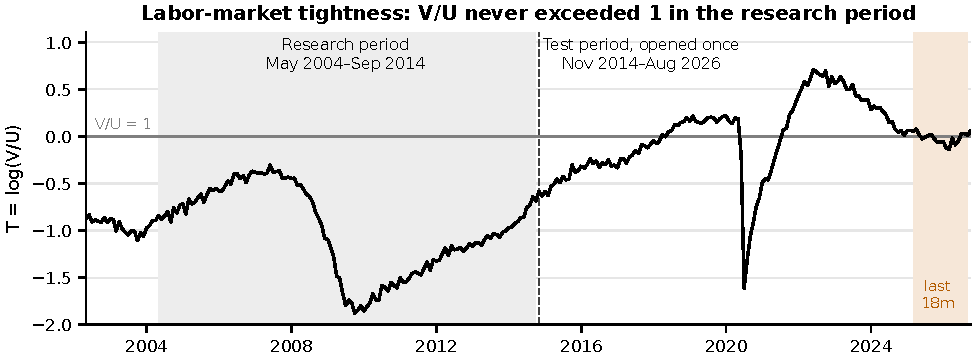
\includegraphics[width=0.58\linewidth]{figures/fig_timeline.pdf}

\caption{Labor-market tightness. Vacancies never exceeded the unemployed in the
research period ($T<0$ throughout), so a tightness effect learned there is
extrapolated in the test.}
\label{fig:tightness}
\end{figure}

% ---------------------------------------------------------------------
% ---------------------------------------------------------------------
\subsection{Implementation: From Signals to Agents}\label{sec:impl}
% ---------------------------------------------------------------------

\subsubsection{From labor flows to signals}
A signal asks a simple question: is this industry hiring (or quitting, or
working longer hours) more than it was a year ago, compared with other
industries? Take the hires rate in construction. We average it over the last
three months available, which smooths out survey noise, and subtract the same
average one year earlier:
\begin{equation}\label{eq:signal}
F_{g,t} = \bar{x}_{g,t-\ell} - \bar{x}_{g,t-\ell-12},
\qquad \bar{x}_{g,t} = \tfrac{1}{3}\left(x_{g,t}+x_{g,t-1}+x_{g,t-2}\right),
\end{equation}
where $x_{g,t}$ is the series for industry group $g$ in month $t$ and $\ell$ is
the publication delay (two months for JOLTS, one for CES). Comparing with the
same months a year earlier removes seasonal patterns and each industry's normal
level. Each month, we then standardise the signal across the 13 industries, so
that only the ranking matters: if every industry hires more, nothing changes.

\subsubsection{Two studies}
We ran two studies on the same data, with the same portfolio, the same rules
and Claude in the loop (Table~\ref{tab:strategies}).

\emph{Study~1} was our first, preregistered pass. It tested the demand channel
(H1): do labor flows predict next month's industry returns? Its signals, models
and pass/fail criteria were fixed before the test period was opened, and the
test was run once. Its primary strategy, A3, adds to a ridge regression
\citep{hoerl1970} the signals proposed by the LLM agents described below. Study~1 did what a
preregistered test is for: it gave a clean answer, no at one month
(Section~\ref{sec:learn}), and its diagnosis showed where to look next.

\emph{Study~2} builds on that diagnosis, as a quant researcher iterates on a
signal. It makes three changes. It brings back wage growth, the only signal with a positive IC in both periods. It lets the research data set the signs that
Study~1 had fixed in advance. And it asks the question the agents of Study~1
were never asked: what do labor flows predict a year ahead, rather than a month?
At twelve months, hires and quits carry the sign the investment channel predicts
(H2), and the resulting book, HQ12 (hires and quits, held twelve months), is
the one we follow. Claude ran this
iteration as an agent, with every stage frozen before it ran. Like any second
iteration, Study~2 is partly fitted to what the first test revealed, so we mark
its results with a dagger (\dag) and validate it the usual way, on new data, in
a forward test.
\begin{table}[H]
\centering
\begin{threeparttable}
\caption{The two studies and their strategies.}
\label{tab:strategies}
\small
\begin{tabularx}{\linewidth}{@{}l >{\raggedright\arraybackslash}X c
  >{\raggedright\arraybackslash}p{0.27\linewidth}@{}}
\toprule
Strategy & What it trades & Holding & Role of the LLM \\
\midrule
\multicolumn{4}{@{}l}{\textit{Study 1, preregistered: demand channel (H1), one-month signals}} \\
A0  & Fixed signs on openings, hires, layoffs and hours & 3 months & none \\
A1  & Ridge regression on the five labor flows           & 3 months & none \\
A1-T & A1, with each flow interacted with tightness      & 3 months & none \\
A3 (primary) & A1 plus the independent agents' features  & 3 months & features proposed by blinded agents \\
A4  & A1 plus the communicating agents' features         & 3 months & same, agents share reports \\
\addlinespace
\multicolumn{4}{@{}l}{\textit{Study 2, post hoc\ph: designed after a post-mortem, run by an iteration agent}} \\
W      & Wage growth                                          & 3 months  & \multirow{4}{=}{\raggedright post-mortem (P5); every stage frozen and run by the iteration agent (P6)} \\
SC     & All six signals, signs estimated on research data   & 3 months  & \\
W+MOM  & Wage growth and 12-month industry momentum           & 3 months  & \\
\textbf{HQ12} & \textbf{Short the industries that hire and quit fastest} & \textbf{12 months} & \\
\bottomrule
\end{tabularx}
\begin{tablenotes}[flushleft]\footnotesize
\item \posthocnote
\end{tablenotes}
\end{threeparttable}
\end{table}

\subsubsection{Portfolio and risk}
Each month we rank the 13 industries on the signal, buy the top three and sell
the bottom three, in equal weights. Each decision is held three months (twelve
for HQ12): the book is the average of the last three (twelve) monthly
portfolios, as in overlapping-portfolio momentum studies \citep{jegadeesh1993}. We hedge its market beta with a position in the market, then scale
the whole book by a single number $k_m$:
\begin{equation}\label{eq:sizing}
k_m \;=\; \min\left\{\, \frac{0.10}{\sqrt{12\,x_m^{\top}\hat\Sigma_m\,x_m}}\;,\;\;
\frac{2}{\sum_{i}\lvert x_{m,i}\rvert} \,\right\},
\qquad w_m = k_m\,x_m ,
\end{equation}
where $x_m$ is the unscaled book (the 13 industry weights and the market hedge)
and $\hat\Sigma_m$ a Ledoit--Wolf covariance estimated over 60 months
\citep{ledoit2004}. The first term targets a volatility of 10\%, the second caps
gross exposure at 2, and the book takes whichever is smaller.

\subsubsection{Turnover and costs}
Turnover is the share of the book traded each month, measured against the
previous weights after they have drifted with returns, so that it counts only
actual trades. We charge 10\,bp per unit of turnover in the industry legs and
2\,bp on the market hedge. HQ12 trades little, since only one twelve-month tranche is replaced
each month: it turns its book over about 4.4 times a year on revised data,
which costs about 0.4\% a year, and it stays profitable up to 50\,bp of trading costs. The
monthly strategies of Study~1 trade about two and a half times as much.
Capacity and the effect of the gross cap are discussed in
Section~\ref{sec:robust}.

\subsubsection{Where the agents come in}
\begin{figure}[H]
\centering
\makebox[\linewidth][c]{%
\begin{tikzpicture}[
  font=\small,
  agent/.style={draw=black!55, fill=black!4, rounded corners=2pt,
                minimum width=1.85cm, minimum height=0.68cm, align=center},
  box/.style={draw=black!60, rounded corners=2pt, align=center,
              inner sep=4pt, font=\footnotesize},
  team/.style={draw=black!45, rounded corners=5pt, inner sep=7pt},
  evalbox/.style={draw=navy, line width=0.8pt, fill=navy!5, rounded corners=2pt,
                  align=center, inner sep=5pt, font=\footnotesize, text width=11cm,
                  execute at begin node={\hyphenpenalty=10000\relax}},
  arr/.style={-{Stealth[length=2mm]}, line width=0.6pt, black!65},
  share/.style={{Stealth[length=1.7mm]}-{Stealth[length=1.7mm]},
                line width=0.8pt, navy},
  note/.style={font=\footnotesize\itshape, text=black!60, align=center}
]
% ---------------- Communicating team ----------------
\node[agent] (c1) at (0,0) {Temporal};
\node[agent, right=0.45cm of c1] (c2) {Composition};
\node[agent, right=0.45cm of c2] (c3) {Interactions};
\draw[share] (c1) -- (c2);
\draw[share] (c2) -- (c3);
\draw[share] (c1.north) to[bend left=20] (c3.north);
\node[font=\small\bfseries, above=0.6cm of c2] (ct) {Communicating team};
\node[note, below=0.14cm of c2] (cn) {reports of at most 120 words after proposals 2 and 4};
\begin{scope}[on background layer]
  \node[team, fit=(c1)(c2)(c3)(ct)(cn)] (C) {};
\end{scope}
% ---------------- Independent team ----------------
\node[agent] (i1) at (8.3,0) {Temporal};
\node[agent, right=0.45cm of i1] (i2) {Composition};
\node[agent, right=0.45cm of i2] (i3) {Interactions};
\node[font=\small\bfseries, above=0.6cm of i2] (it) {Independent team};
\node[note, below=0.14cm of i2] (in) {no exchange};
\begin{scope}[on background layer]
  \node[team, fit=(i1)(i2)(i3)(it)(in)] (I) {};
\end{scope}
% ---------------- Evaluator ----------------
\coordinate (mid) at ($(C.south)!0.5!(I.south)$);
\node[evalbox, below=1.25cm of mid] (E)
  {\textbf{Blinded evaluator}: research data only; variables V01--V06,
   groups G01--G13, no dates. Returns the IC, its $t$-statistic, coverage,
   correlation with earlier proposals, and the IC in each tightness regime.};
\foreach \T in {C,I}{
  \draw[arr] ([xshift=-5mm]\T.south) -- node[left, note]{proposals}
             ([xshift=-5mm]\T.south |- E.north);
  \draw[arr] ([xshift=5mm]\T.south |- E.north) -- node[right, note]{feedback}
             ([xshift=5mm]\T.south);
}
% ---------------- Selection and strategies ----------------
\node[box, below=0.7cm of E] (S)
  {\textbf{Mechanical selection, run 1 only}\\
   $t\geq1.5$, same sign in both halves, low correlation};
\draw[arr] (E) -- (S);
\node[box, below=0.85cm of S.south west, anchor=north] (A4)
  {\textbf{A4} = ridge + features\\of the communicating team};
\node[box, below=0.85cm of S.south east, anchor=north] (A3)
  {\textbf{A3} (primary) = ridge +\\features of the independent team};
\draw[arr] (S.south) -- ++(0,-0.35) -| (A4.north);
\draw[arr] (S.south) -- ++(0,-0.35) -| (A3.north);
% ---------------- Judge (left) and runs note (right) ----------------
\node[box, anchor=north west] (J) at (C.south west |- S.north) {\textbf{LLM judge}:\\was a reported\\idea reused?};
\node[box, below=0.45cm of J] (H) {\textbf{Human audit}\\of a sample};
\draw[arr, dashed] (J.north |- C.south) -- (J.north);
\draw[arr] (J) -- (H);
\end{tikzpicture}
}
\caption{The agent experiment. Two teams of three agents with the same budget of
six proposals each: one shares short reports, the other does not. Neither can see
the evaluator, the names of the variables or the dates. The design is run three
times; runs 2 and 3 only measure how much of the search is luck.}
\label{fig:islands}
\end{figure}

Figure~\ref{fig:islands} shows the agent experiment. Six autonomous agents
propose new signals from the labor data. They are split into two teams of three,
with the same budget of six proposals each. Each agent has one goal, stated in
its prompt: find a formula that ranks the thirteen industries in the same order
as their returns over the next month. The agent never sees the data or the
returns. It sees only a short dictionary of the six labor variables under
anonymous names (V01 to V06) with their units, the labels G01 to G13 for the
industries, and no dates, so it cannot recall what happened to any real
industry. A proposal is a short formula, much like a spreadsheet formula, built
from a fixed menu of 14 operations such as changes, ratios, rankings and
conditions on the state of the labor market (Appendix~\ref{app:grammar}). For
example, \texttt{yoy(V05)} is the change in variable V05 over the past year. Each
proposal goes to an evaluator, a program the agents can neither read nor modify.
It computes the formula for every industry and month of the research period,
and returns a short score. The main number is the information coefficient (IC):
each month, the correlation between the ranking given by the formula and the
ranking of next month's industry returns, averaged over the research period.
The score also gives the IC's $t$-statistic, how often the signal was active,
how close it is to earlier proposals, and its IC in each tightness regime. The
agent's task is to raise this score, and it uses each score to decide what to
try next. The two teams differ in one thing: after their second and fourth
proposals, agents in the communicating team write a short report on what
worked, and the others read it before proposing again. This is the island model
of Section~\ref{sec:ideas}, and it asks whether sharing helps.


A fixed rule then selects, from the first of three runs, the features that are
significant, stable over the research period and not redundant. The
independent team's features enter the primary strategy (A3), the communicating
team's enter A4. The second and third runs only measure how much of the search
is luck. Separately, an LLM judge reads each report and the proposals that
follow it to decide whether an idea was reused, and a person checks a sample of
its decisions. We ran the experiment with Claude Sonnet (Study~1), and again
with Claude Opus after the test had been opened (Study~1b).

In total, Claude played six roles, numbered in the order they occurred: P1,
an audit of the data and code before any result existed; P2, the signal agents
described above; P3, the judge; P4, a red team of the research results; P5, a
post-mortem of Study~1; and P6, the iteration agent that rebuilt the analysis
and ran Study~2 under a written rules file. Section~\ref{sec:ai} evaluates each.

\begin{protocolbox}
\begin{itemize}[leftmargin=1.1em]
\item \textbf{Same rules for both studies.} Every input as known on the
  decision date; every specification frozen and hashed before it ran; every
  result reported whatever its sign; Sharpe ratios deflated for every look taken
  \citep{bailey2014}.
\item \textbf{Study~1 is confirmatory.} Its signals, models, primary strategy and
  five pass/fail gates were frozen before any test data were touched, and the
  test was opened once. We verified the freeze record against the repository.
\item \textbf{Study~2 is post hoc.} It was designed after the test was opened,
  so its test results cannot validate it. Its results carry a dagger (\dag),
  and only the forward test can confirm them.
\end{itemize}
\end{protocolbox}

\subsubsection{Prompts}
Three prompts cover idea generation, coding support and robustness design. All
are verbatim; outputs and our evaluation are in Section~\ref{sec:ai}, transcripts
and the rules that governed the iteration agent in Appendix~\ref{app:claude}.

\begin{promptbox}{Idea generation: blinded signal agent (P2)}{system prompt, opening}
You are a quantitative researcher. You will propose one feature per turn to
predict which of 13 anonymous groups (G01 to G13) will have higher returns next
month relative to the others. You see only the variable dictionary below, the
allowed operations, and summary statistics of your previous submissions. You do
not know what the groups, variables or time periods are. Do not guess them and
do not use knowledge about any real industry, company or date. [variable
dictionary, grammar and JSON format follow]
\end{promptbox}

\begin{promptbox}{Coding support: data and code audit (P1)}{user prompt}
Find mapping errors, timestamp or look-ahead errors, and code bugs in the
material below. For each problem, give the exact line or row, why it is wrong,
and a test that would confirm it. Do not report style issues. [followed by the
series manifest, the industry crosswalk and the as-of code]
\end{promptbox}

\begin{promptbox}{Robustness design: red team (P4)}{user prompt}
Give 10 distinct reasons these results could be spurious, ranked by likelihood.
For each, name a test that can be run with this data and the result that would
make us say "do not implement". [followed by the research-period result tables,
without dates or names]
\end{promptbox}




\newpage



\section{What We Learned: Results}\label{sec:learn}

\begin{answerbox}
\begin{itemize}[leftmargin=1.1em]
\item \textbf{H1, demand channel: rejected.} The preregistered one-month
  strategies did not predict industry returns; the primary strategy's forecasts
  did no better than a placebo ($p=0.72$).
\item \textbf{H2, slow cost channel: promising, not established\ph.} Shorting
  the industries that hire and quit fastest for twelve months (HQ12) earns a
  test Sharpe ratio of $+0.20$ on data as known and is positive in every
  window. It was designed after the test was opened.
\item \textbf{H3, tightness: untestable as designed.} Vacancies never exceeded
  the unemployed in the research period.
\item \textbf{Agents: discipline without discovery.} They followed the
  protocol, better with a stronger model, but none of their signals survived the
  test, and our explanations of their failures did not hold up when tested.
\end{itemize}
\end{answerbox}

\begin{table}[H]
\centering
\begin{threeparttable}
\caption{Net Sharpe ratios on data as known: the one-time test and the windows
the brief asks for.}
\label{tab:main}
\small\setlength{\tabcolsep}{6pt}
\begin{tabular}{@{}l r r r r r@{}}
\toprule
 & Research & \textbf{Test} & Full & Post-2010 & Last 18m \\
\midrule
\multicolumn{6}{@{}l}{\textit{Study 2, post hoc\ph}} \\
\textbf{HQ12} hires and quits, 12 months & $+0.54$ & $\mathbf{+0.20}$ & $+0.31$ & $+0.23$ & $+0.14$ \\
W wage growth                     & $+0.11$ & $+0.13$ & $+0.13$ & $+0.10$ & $-1.31$ \\
W+MOM wage growth and momentum    & $+0.25$ & $+0.46$ & $+0.37$ & $+0.31$ & $-0.94$ \\
SC signed composite               & $+0.34$ & $+0.24$ & $+0.28$ & $+0.12$ & $+1.38$ \\
\addlinespace
\multicolumn{6}{@{}l}{\textit{Study 1, preregistered: the one-time test}} \\
A3 agent features (primary)       & $-0.13$ & $-0.58$ & $-0.44$ & $-0.62$ & $+0.85$ \\
A4 communicating agents           & $-0.18$ & $-0.79$ & $-0.56$ & $-0.74$ & $+1.23$ \\
\bottomrule
\end{tabular}
\begin{tablenotes}[flushleft]\footnotesize
\item Annualised, net of 10\,bp industry and 2\,bp hedge costs, labor data as
published on each decision date. Test: November 2014 to August 2026 (142
months); last 18 months: March 2025 to August 2026. For Study~1, the research
column uses the 88 months in which every model had a forecast, and the full
sample starts in June 2007. On revised data, HQ12's test Sharpe ratio is
$+0.29$. A0, A1 and A1-T are in Appendix~\ref{app:study1}. \posthocnote
\end{tablenotes}
\end{threeparttable}
\end{table}

% ---------------------------------------------------------------------
\subsection{Style and Risk Exposures: What Else the Books Hold}\label{sec:style}
% ---------------------------------------------------------------------
We regress each book's net return on the five Fama--French factors
\citep{famafrench2015}, momentum \citep{carhart1997} and industry momentum (full
loadings in Appendix~\ref{app:study2}). HQ12 is
short profitability (RMW $-0.36$, $t=-4.5$, revised data): shorting the industries that hire
and quit fastest means shorting profitable, growing industries. It does not
load on the investment factor (CMA), so it is not the known investment premium
in disguise, and its alpha is positive but not significant ($+0.16\%$ a month
on data as known, $t=0.92$). Study~1's primary strategy leaned the other way,
long profitability (RMW $+0.19$). \textbf{For Q1,} what labor flows capture beyond
profitability is positive but too small to measure with confidence.

% ---------------------------------------------------------------------
\subsection{Performance over Time: Positive Everywhere, Not Every Year}\label{sec:time}
% ---------------------------------------------------------------------
HQ12 is positive in every window of Table~\ref{tab:main}: $+0.31$ over the
full sample, $+0.23$ after 2010 and $+0.14$ over the last 18 months. So is the
signed composite, but its signs change with the data version, so we read little
into it. These windows hide an uneven path, however. Within the test, HQ12 lost
money in its first half (2014 to 2020, $-0.23$) and more than made it back in
the second ($+0.49$); the longer windows are positive because the later gains
outweigh that loss. Wage growth worked until 2024 and
lost heavily over the last 18 months ($-1.31$). Study~1 lost over the
full sample and after 2010, and its gain over the last 18 months rests on an IC
that is statistically zero ($t=0.44$). Industry momentum, the benchmark to
beat, earned $+0.03$ over the test. \textbf{For Q1,} the slow hiring signal is the only stable one across windows,
and only half of the test supports it.

% ---------------------------------------------------------------------
\subsection{Robustness and Limits: Why the Demand Channel Failed, What Might Survive}\label{sec:robust}
% ---------------------------------------------------------------------

\subsubsection{Why the demand channel failed}
Study~1's answer holds. Its primary strategy stays negative under every data
version, cost level, dropped industry, gross cap and weighting scheme, and in
every sub-period except the last 18 months; its 90\% block-bootstrap interval \citep{kunsch1989}, $[-0.99,-0.16]$,
excludes zero; its forecasts did no better than a placebo; and no preregistered
strategy beat another once corrected for multiple comparisons \citep{holm1979}. The diagnosis has four parts, each
addressed by Study~2. Layoffs and hours carried the opposite sign to the one
imposed. Hiring predicts nothing at one month, but lower returns at twelve. The
slack regime that H3 relied on occurred in 3 of 142 test months. And the two
agent features of the primary strategy were active only in those months. The
warning signs were already visible on research data, where every Study~1
strategy had a negative Sharpe ratio and cross-validation chose the strongest
penalty for every model.

\subsubsection{What might survive: a slow cost channel\ph}
HQ12's sign is the one the investment channel predicts \citep{belo2014}. Its
twelve-month horizon, however, was chosen from a profile that included the
test: on research data alone, its twelve-month IC is not significant, and that
sample would not have selected it. Figure~\ref{fig:horizon} shows the profile:
nothing at one month, a positive IC from nine to 24 months. On data as known,
HQ12 passes six of the seven checks declared before its battery ran, and fails
one: the first half of the test lost money (Table~\ref{tab:battery}). Its alpha and deflated
Sharpe ratio remain far from the thresholds declared with the variants. The
other variants are weaker: W has no alpha, W+MOM draws its return from
momentum, and SC's signs depend on the data version.

\begin{figure}[H]
\centering
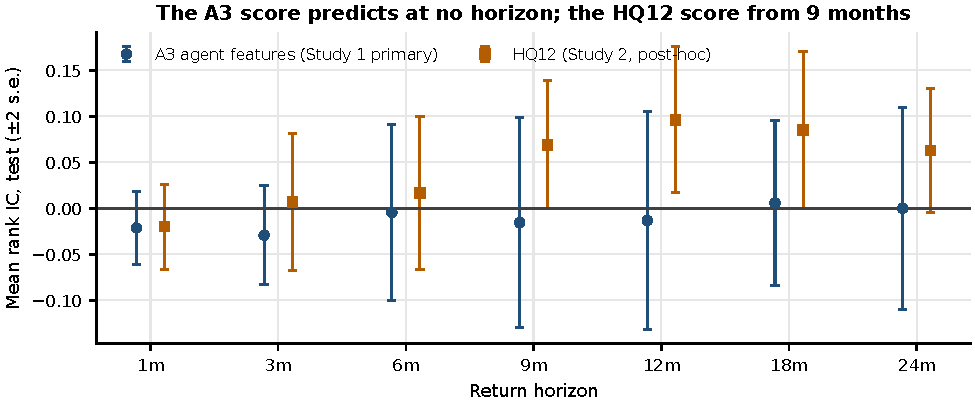
\includegraphics[width=0.58\linewidth]{figures/fig_s1_horizon.pdf}

\caption{Where each score predicts. The primary score of Study~1 has no IC at
any horizon; the HQ12 score has none at one month and a positive IC from nine
months on. Revised data.\ph}
\label{fig:horizon}
\end{figure}

\begin{table}[H]
\centering
\begin{threeparttable}
\caption{HQ12 robustness battery, data as known, test window unless stated.}
\label{tab:battery}
\small
\begin{tabularx}{\linewidth}{@{}X l c@{}}
\toprule
Check (declared before the battery ran) & Result & Met \\
\midrule
Each component alone, held 12 months (Sharpe): hires; quits & $+0.19$; $+0.17$ & yes \\
12-month IC ($t$); 1-month IC $t$                            & $+0.085$ ($2.26$); $-0.42$ & yes \\
Holding 9 and 18 months (Sharpe)                             & $+0.16$; $+0.11$ & yes \\
Both test halves positive                                    & $-0.23$; $+0.49$ & no \\
Break-even trading cost above 25\,bp                         & 50\,bp & yes \\
Drop one industry: lowest and highest Sharpe                 & $+0.05$; $+0.36$ & yes \\
Bootstrap 90\% interval excludes zero: test; full sample     & $[-0.14,+0.57]$; $[+0.02,+0.60]$ & yes (full) \\
\addlinespace
\multicolumn{3}{@{}l}{\textit{From the reading rule declared with the variants}} \\
Factor alpha $t$ (test; full sample)                         & $0.92$; $1.81$ & no \\
Deflated Sharpe ratio (162 looks)                            & $0.02$ & no \\
\bottomrule
\end{tabularx}
\begin{tablenotes}[flushleft]\footnotesize
\item Newey--West standard errors \citep{neweywest1987}: 12 lags for the alpha,
$h+5$ for ICs at horizon $h$. \posthocnote
\end{tablenotes}
\end{threeparttable}
\end{table}

\subsubsection{Limits}
Even a genuine signal could not have earned much here. The fundamental law of
active management \citep{grinold1989,clarke2002} links the information ratio
to the quality of each bet (IC), the number of independent bets per year (BR)
and the share of the signal that reaches the portfolio (TC):
\begin{equation}\label{eq:flaw}
IR \;\approx\; IC \times \sqrt{BR} \times TC .
\end{equation}
The 13 industries behave like nine independent bets, so a monthly book has
$BR\approx 9\times12=108$, and even a good IC of 0.05 caps the ratio near 0.5.
HQ12 renews its bets once a year across about ten effective industries
($BR\approx10$) and passes about half of its signal to the portfolio
($TC\approx0.48$), so the law implies $0.085\times\sqrt{10}\times0.48\approx0.13$.
That is the same order as the $+0.20$ it realised and well within sampling
error, since a Sharpe ratio measured over 142 months has a standard error of
about 0.3: the result is not too good to be true. Capacity is small (about \$1.2 million before trading reaches
1\% of the least liquid ETF's daily volume), and the gross cap binds in most
months without hurting the Sharpe ratio. H3 could not be tested,
HQ12's horizon was chosen with the test in view, the agents searched only at one
month, and with 142 months only a Sharpe ratio near 0.6 reaches $t\approx2$. The
forward test frozen on 3 October 2026 (Appendix~\ref{app:forward}) holds one
tranche for a quarter, where HQ12 shows no IC; only that tranche's twelve-month
return will be informative.

\textbf{Answer to Q1.} Labor flows do not predict which industries outperform over the next
month. Over the next year, the data are consistent with the investment channel,
but the evidence is post hoc and short of significance.

% ---------------------------------------------------------------------
\subsection{Evaluating the AI Research Assistant: Discipline without Discovery}\label{sec:ai}
% ---------------------------------------------------------------------
Claude took every AI role: Sonnet 5.5 for the 199 calls of Study~1, Opus 5.5 for
the 294 calls of Study~1b, and later Claude models for the post-mortem and the
iteration. Each interaction is documented, with transcripts and our
critiques, in Appendix~\ref{app:claude}. Its six roles, numbered P1 to P6 in the order they occurred, are defined in
Section~\ref{sec:impl}; we evaluate Claude as an assistant, as a researcher and
as a judge.

\subsubsection{Claude as assistant: a useful auditor that moves the goalposts}
The audit of the data and code (P1) caught every real gap in the mapping, but
five of its 25 findings were claims the files did not support, and it presented
design choices as ``confirmed errors''. The red team (P4) read the research
tables correctly, yet asserted a $p$-value it had never computed and proposed
new pass/fail thresholds after seeing the results. Both errors are typical of
language models: they can state with confidence what they have not checked, a
failure known as hallucination \citep{ji2023}, and specialised quantitative work
leaves little room for it. The post-mortem (P5) found the right cause
of Study~1's failure, but its fixes were read off the test results, and the wage
signal it called stable lost heavily over the last 18 months. We checked every
finding, kept the registered tests and labelled every later change post hoc.

The iteration agent (P6) is the counter-example, and the clearest gain. It
rebuilt the analysis, reproduced Study~1's returns to $10^{-16}$, ran every stage
of Study~2 with each number tied to the file it comes from, and froze each stage
before running it, work that would have taken us far longer by hand. When
it wrongly assumed that August JOLTS data would not be out by 29 September, its
own pre-committed check stopped the run. \textbf{The difference lies in the setting,
not the model:} the red team and the post-mortem could change the rules, the
iteration agent could not, because its rules were enforced by code rather than
stated in a prompt.

\subsubsection{Claude as researcher: protocol followed, nothing found}
The agents followed the blind protocol, and a stronger model followed it better
(Table~\ref{tab:agents}): no call tried to recover the hidden names or dates,
and Opus made more valid proposals than Sonnet. Neither found a signal
that survived. A feature's research IC barely predicts its test IC
(Figure~\ref{fig:agentic}), and none of the eight selected features met the test
criterion, though two of Opus's kept a small positive test IC. \textbf{A stronger model improved discipline, not discovery.}

\begin{table}[!htb]
\centering
\caption{The agents in numbers: a stronger model followed the protocol better and
found no more signal.}
\label{tab:agents}
\small
\begin{tabular}{@{}l c c@{}}
\toprule
 & Study 1 (Sonnet 5.5) & Study 1b (Opus 5.5)\ph \\
\midrule
Valid proposals                              & 98 / 108 & 106 / 108 \\
Reports admitted (communicating team)        & 7 / 18   & 15 / 18 \\
Usable judge answers                         & 8 / 36   & 84 / 88 \\
Correlation of research and test IC          & 0.22     & 0.37 \\
Selected features meeting the test criterion & 0 / 4    & 0 / 4 \\
\bottomrule
\end{tabular}
\end{table}

\begin{figure}[!htb]
\centering
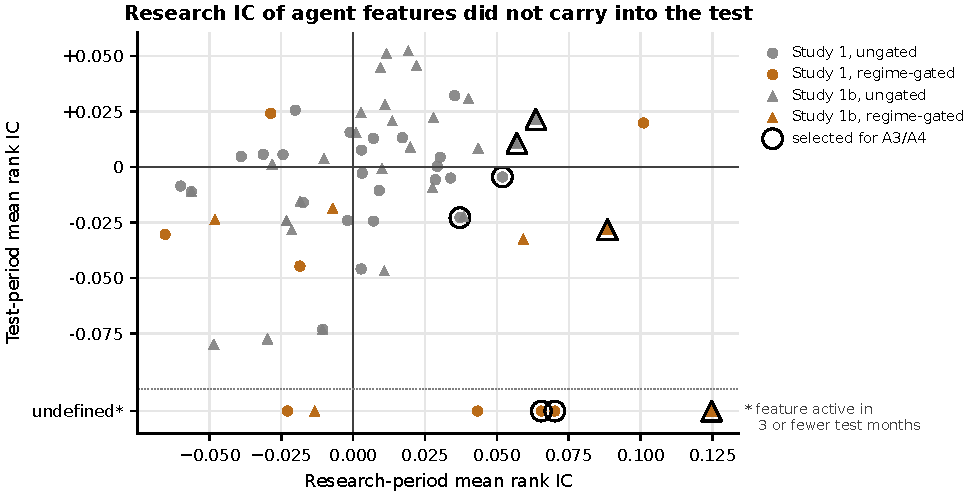
\includegraphics[width=0.75\linewidth]{figures/fig_agents_scatter.pdf}


\caption{Research IC of agent features barely predicts their test IC. The
selected regime-gated features were active in 3 test months.\ph}
\label{fig:agentic}
\end{figure}

\subsubsection{Islands: no detectable gain from sharing}
The island model is the most distinctive part of our design
(Section~\ref{sec:ideas}). \textbf{In our setting, sharing had no detectable effect.} In
both studies, the gap in best research IC between the communicating and the
independent team lies within the spread across the three runs (permutation
$p=0.30$ for Sonnet and $0.10$ for Opus; Appendix~\ref{app:study2}). Two details matter. With Sonnet,
sharing barely happened: 11 of 18 reports were rejected, mostly for running over
120 words. With Opus, which delivered 15 of 18 reports, the communicating team
did better in all three runs, the most extreme ordering three runs allow. Sharing
may therefore help a model that follows the exchange protocol, but three runs
cannot tell. Our setting was also unfavourable to islands: they pay off when
parallel searches tackle different problems and have something worth passing
on, whereas our two teams searched the same problem for a signal that may not
exist.

\subsubsection{Claude as judge, and testing our own explanations}
To measure whether ideas spread, an LLM judge read each report and the
proposals that followed it (P3). It overstated uptake: on the 17 Opus pairs we
checked by hand, it said an idea had been reused 10 times and the human 3
times, and all seven disagreements were false yeses. It matched vocabulary
rather than content.

Our critiques proposed two explanations, each with a fix, and we tested both.
If the judge matches vocabulary, requiring it to quote the exact claim it relies
on should help: it fixed the format of Sonnet's answers (8 of 8 usable, against
2 before) but not Opus's judgment, which still said yes falsely 8 times in 17.
If the agents built regime gates because their feedback showed the IC in each
tightness regime, removing that split should remove the gates: it did not (4 of
48 valid proposals with the split, 3 of 50 without). The rerun produced fewer
gates than the original study, so this test is weak, but it gives no support to
our explanation. The selection data point to another one: gated features were
measured on 43 to 48 consecutive research months, against 120 or more for the
others, and they were overrepresented among the selected features (2 of 4 in
each study, against 9 of 33 and 6 of 35 among the candidates). The selection
rule, not the feedback, may have rewarded them. \textbf{Our first explanations of the
agents' behaviour were plausible, and they did not survive a test.}

Next time, we would require a minimum of active months for selection, check
the judge's quotes by text search, search at several horizons and run more
repetitions.

\textbf{Answer to Q2.} An LLM assistant helped wherever
the protocol kept it away from the results, and every claim about its
behaviour, including our own, had to be tested.
\vspace{0.5cm}

% =====================================================================
\section{Conclusion}\label{sec:conclusion}
We asked two questions.

\emph{Q1: do labor-market flows predict which U.S. industries outperform, net of
costs and risk?} \textbf{Not over the next month.} Study~1, preregistered and tested once
on 142 months, found no predictive power, and that answer holds under every
check. Over the next year, the data are consistent with the investment channel:
the industries that hire and lose workers fastest earned lower returns, and
HQ12, which shorts them, earned a Sharpe ratio of $+0.20$ on data as known. But
this was found after the test was opened, and it does not survive a correction
for the number of looks taken. We conclude: \textbf{do not implement}, and
follow HQ12 out of sample, at its own twelve-month horizon.

\emph{Q2: how should an LLM research assistant be integrated so that it helps
without misleading us?} \textbf{By giving it the parts of research it does well and
keeping it away from the results.} Claude was a fast, wide auditor and a
disciplined signal searcher, and a stronger model was more disciplined still.
But it found nothing that survived the test, it moved the goalposts whenever it
saw results, and it was an unreliable judge of its own agents. What made it
useful was the protocol around it: blinding, an evaluator out of its reach,
frozen specifications and human checks. And when we tried to explain its
failures, our own explanations did not survive testing either. Claims about how
an AI behaves need the same out-of-sample discipline as claims about alpha.

Three extensions follow. Stock-level baskets built from NAICS codes would give
the signal far more independent bets than thirteen industries. Agents asked to
search at several horizons could test what Study~1's agents were never asked.
And the HQ12 tranche bought on 30 September 2026 should be evaluated after its
full twelve months, not after one quarter.

\newpage

% =====================================================================
\bibliography{references}
% =====================================================================

% =====================================================================
% =====================================================================
% Appendices
% =====================================================================
\clearpage
\appendix
\crefalias{section}{appendix}
\crefalias{subsection}{appendix}
\titleformat{\section}
  {\normalfont\large\bfseries\headcolor}{Appendix \thesection.}{0.6em}{}
\renewcommand{\thesection}{\Alph{section}}

\section{Names used in this report}\label{app:names}
% ---------------------------------------------------------------------
\noindent\textbf{Repository.} Code, data-building scripts, frozen specifications,
run logs and every table and figure of this report:
\url{https://github.com/pieropls/MFE230GA}.

The repository and the result files were renamed on 4 October 2026. Result
files frozen before that date keep the old codes inside, so they stay
byte-identical.

\begin{table}[H]
\centering\footnotesize
\caption{Name mapping.}
\begin{tabularx}{\textwidth}{@{}p{4.6cm} X@{}}
\toprule
Old name & Name in this report \\
\midrule
frozen, sealed or Sonnet study & Study 1: preregistered (Alex), folder \path{study1_preregistered/} \\
Opus follow-up & Study 1b: exploratory follow-up (Opus) \\
v2, v3, v4 runs & Study 2: post-hoc iteration; 2.1 variants (was v2), 2.2 robustness of HQ12 (was v3), 2.3 additional robustness (was v4) \\
A0, A1, A1-T, A3, A4 & A0 fixed rule; A1 ridge; A1-T ridge $\times$ tightness; A3 agent features, independent (primary); A4 agent features, communicating \\
V2a, V2b, V2c, V2d & W wage growth; SC signed composite; W+MOM wage growth and momentum; HQ12 hires and quits, held twelve months \\
P1 to P6 & P1 data and code audit; P2 signal agents; P3 judge; P4 red team; P5 post-mortem review; P6 iteration agent \\
islands, sealed test, F1--F5 & communicating team; one-time test; openings, hires, quits, layoffs, hours \\
\bottomrule
\end{tabularx}
\end{table}

% ---------------------------------------------------------------------
\section{Study 1 in full: preregistered (Alex)}\label{app:study1}\label{app:results}
% ---------------------------------------------------------------------
Everything in this section labelled confirmatory is read from Study~1's saved
files and is unchanged: \path{results.json} and the ledgers next to it, under
\path{study1_preregistered/outputs/follow_the_workers/outputs/sealed/initial/}.
The diagnostics labelled post hoc were computed afterwards from the same saved
files and public data.

\subsection*{Design}
Thirteen industry groups (\cref{app:mapping}); signals F1--F5 as known at each
decision date; five strategies (\cref{tab:strategies}); research May 2004 to
September 2014, test November 2014 to August 2026; top three against bottom
three, three monthly tranches, beta hedge, 10\% volatility target, gross cap 2,
10\,bp and 2\,bp costs. Five gates decide the verdict for the primary: G1 timing
(pass), G2 prediction (IC $t\ge2$; fail), G3 incremental alpha ($t\ge2$; fail),
G4 robustness (positive IC in both halves, placebo $p<0.05$, no industry above
half the profit; fail), G5 implementable (Sharpe $>0$ at 25\,bp, capacity
documented; fail). % src: claim C07
The freeze record was checked against the files (\cref{tab:freeze}). % src: claims B01, B02
The score-to-weight mapping, with $s_{m,g}$ the score of group $g$ known at the
end of month $m-1$, is below; \cref{eq:sizing} in the main text is its scaling
step.
% Score-to-weight mapping of the frozen study's backtest (study1_preregistered/outputs/follow_the_workers/data.py::backtest).
% Written by analysis/run.ipynb. Parameters: analysis/params.py PORTFOLIO (checked equal to the frozen params in Gate 1).
\begin{align}
\tau_{m,g} &= \begin{cases} +\tfrac13 & g \in \text{top 3 of } s_{m,\cdot}\\ -\tfrac13 & g \in \text{bottom 3 of } s_{m,\cdot}\\ 0 & \text{otherwise}\end{cases}
  \qquad b_{m} = \frac{1}{H}\sum_{j=0}^{H-1} \tau_{m-j}, \quad H=3, \label{eq:tranche}\\
h_{m} &= -\sum_{g} b_{m,g}\,\hat\beta_{m,g}, \qquad x_m = (b_{m,1},\dots,b_{m,13},\,h_m), \label{eq:hedge}\\
k_m &= \min\!\left(\frac{0.10}{\sqrt{12\,x_m^{\top}\hat\Sigma_m x_m}},\ \frac{2}{\lVert x_m\rVert_1}\right), \qquad w_m = k_m\,x_m, \label{eq:scale}\\
r^{\mathrm{net}}_{m} &= \sum_{g} w_{m,g}\, r^{e}_{m,g} + w_{m,M}\,\mathrm{MKT}_m
  - c\sum_{g}\lvert w_{m,g}-\tilde w_{m,g}\rvert - c_h\,\lvert w_{m,M}-\tilde w_{m,M}\rvert. \label{eq:net}
\end{align}
where $s_{m,g}$ is the score of group $g$ known at the end of month $m-1$, $\hat\beta_{m,g}$ and the Ledoit--Wolf covariance
$\hat\Sigma_m$ (13 groups plus the market) use the 60 months ending in $m-2$ (at least 36), $r^{e}_{m,g}$ is the group's excess
return, $\tilde w$ are the previous weights after drift, $c=10$\,bp and $c_h=2$\,bp.


\begin{table}[H]\centering\footnotesize\caption{Study 1: all five strategies in the test window. \hfill\tagc}\setlength{\tabcolsep}{4pt}\fit{% CONFIRMATORY (A0-A4) / POST-HOC (momentum) | source: analysis/output/study1/tables/d4_test_performance.csv (generated by analysis/run.ipynb)
\begin{tabular}{lrrrrrr}
\toprule
strategy & Sharpe & Net p.a. & Vol. & Max DD & Turnover & Costs p.a. \\
\midrule
A0 fixed rule & $-$0.36 & $-$3.5\% & 9.7\% & $-$40.3\% & 0.83 & 1.01\% \\
A1 ridge & $-$0.51 & $-$4.0\% & 7.9\% & $-$37.7\% & 0.91 & 1.11\% \\
A3 primary & $-$0.58 & $-$4.6\% & 7.8\% & $-$41.1\% & 0.91 & 1.11\% \\
A4 island agents & $-$0.79 & $-$6.1\% & 7.8\% & $-$53.3\% & 1.11 & 1.35\% \\
Industry momentum 12-1 & +0.03 & +0.3\% & 9.4\% & $-$20.8\% & 0.53 & 0.65\% \\
\bottomrule
\end{tabular}
}\end{table}
\begin{table}[H]\centering\scriptsize\caption{Study 1 robustness, full table: the four data versions, costs, sub-periods, drop-one-group, gates, and the diagnostics added in Study 2.3. \hfill\tagc\ / \tagp\ (last four rows)}\setlength{\tabcolsep}{4pt}\fit{% CONFIRMATORY / POST-HOC | source: analysis/output/study1/tables/d11_study1_robustness.csv (generated by analysis/run.ipynb)
\begin{tabular}{p{6.1cm}p{5.0cm}p{3.6cm}}
\toprule
Check (test window, as-known data unless stated) & A3 agent features (primary) & A0 fixed rule \\
\midrule
Test Sharpe, data as known & $-$0.58 & $-$0.36 \\
Test Sharpe, data first release & $-$0.52 & $-$0.16 \\
Test Sharpe, data revised & $-$0.56 & $-$0.26 \\
Test Sharpe, data fixed lag & $-$0.53 & $-$0.27 \\
Net return p.a. & $-$4.6\% & $-$3.5\% \\
IC, one month (t) & $-$0.021 ($-$1.08) & $-$0.020 ($-$0.71) \\
Factor alpha per month (t) & $-$0.38\% ($-$1.86) & $-$0.25\% ($-$0.92) \\
Placebo p (circular shift) & 0.72 & n/a (primary only) \\
Holm-adjusted p, IC and return & 1.00, 1.00 (A3 vs A1) & 1.00, 1.00 (A1 vs A0) \\
Deflated Sharpe, research (41 trials) & 0.003 & 0.000 \\
Sharpe at 0 / 10 / 25 bp & $-$0.45 / $-$0.58 / $-$0.79 & n/a / $-$0.36 / n/a \\
Sharpe, first test half & $-$0.72 & $-$0.55 \\
Sharpe, second test half & $-$0.49 & $-$0.20 \\
Sharpe, excluding Mar-Dec 2020 & $-$0.51 & $-$0.18 \\
Sharpe, last 18 months & +0.85 & $-$1.56 \\
Drop one group, Sharpe range & $-$0.70 (Wholesale) to $-$0.24 (Durable mfg) & n/a (primary only) \\
Gates G1 timing / G2 prediction / G3 alpha / G4 robustness / G5 implementable & pass / fail / fail / fail / fail & n/a (primary only) \\
Verdict & Do not implement & not primary \\
Block-bootstrap 90\% interval, test Sharpe & [$-$0.99, $-$0.16] & [$-$0.91, +0.20] \\
A3 score IC at 1 / 6 / 12 / 24 months (t) & $-$0.021 ($-$1.08) / $-$0.004 ($-$0.09) / $-$0.013 ($-$0.22) / $-$0.000 ($-$0.00) & n/a \\
A3 Sharpe with cap 2 / cap 3 / no cap & $-$0.58 / $-$0.61 / $-$0.62 & n/a \\
A3 Sharpe, rank-weighted book & $-$0.49 & n/a \\
\bottomrule
\end{tabular}
}\end{table}
\begin{table}[H]\centering\scriptsize\caption{Risk overlay of every Study 1 and Study 1b strategy: how often the cap bound, ex-ante and realised volatility. \hfill\tagc}\setlength{\tabcolsep}{4pt}\fit{% POST-HOC | source: analysis/output/study1/tables/d9_risk_overlay.csv (generated by analysis/run.ipynb)
\begin{tabular}{lrrrrr}
\toprule
Study, strategy & Cap binds & Ex-ante vol & Realised vol & Gross leverage & |Hedge| \\
\midrule
Study 1 A0 & 80\% & 8.0\% & 9.7\% & 1.96 & 0.15 \\
Study 1 A1 & 88\% & 7.5\% & 7.9\% & 1.98 & 0.13 \\
Study 1 A1-T & 82\% & 7.5\% & 8.2\% & 1.97 & 0.12 \\
Study 1 A3 & 87\% & 7.5\% & 7.8\% & 1.98 & 0.13 \\
Study 1 A4 & 91\% & 7.3\% & 7.8\% & 1.99 & 0.13 \\
Study 1b A3 & 92\% & 7.3\% & 7.5\% & 1.99 & 0.15 \\
Study 1b A4 & 93\% & 7.3\% & 8.4\% & 1.99 & 0.11 \\
\bottomrule
\end{tabular}
}\end{table}
\begin{table}[H]\centering\scriptsize\caption{Factor loadings of the Study 1 books (FF5, momentum, industry momentum). \hfill\tagc}\setlength{\tabcolsep}{4pt}\fit{% CONFIRMATORY | source: analysis/output/study1/tables/d6_factor_loadings.csv (generated by analysis/run.ipynb)
\begin{tabular}{lrrr}
\toprule
Factor & A0 fixed rule & A1 ridge & A3 primary \\
\midrule
Alpha (per month) & $-$0.25\% ($-$0.92) & $-$0.35\% ($-$1.72) & $-$0.38\% ($-$1.86) \\
Market & $-$0.01 ($-$0.31) & $-$0.01 ($-$0.20) & $-$0.03 ($-$0.43) \\
SMB & +0.02 (+0.21) & +0.12 (+1.01) & +0.10 (+0.89) \\
HML & +0.09 (+0.60) & $-$0.15 ($-$1.97) & $-$0.15 ($-$2.01) \\
RMW & +0.00 (+0.05) & +0.21 (+2.33) & +0.19 (+2.16) \\
CMA & $-$0.04 ($-$0.21) & +0.05 (+0.47) & +0.03 (+0.26) \\
Momentum & $-$0.06 ($-$0.72) & +0.01 (+0.15) & $-$0.01 ($-$0.17) \\
Industry momentum & +0.22 (+1.93) & $-$0.02 ($-$0.21) & $-$0.01 ($-$0.12) \\
\bottomrule
\end{tabular}
}\end{table}
\begin{table}[H]\centering\scriptsize\caption{Freeze record, checked against the files in the repository. \hfill\tagc}\label{tab:freeze}\setlength{\tabcolsep}{4pt}\fit{% CONFIRMATORY | source: analysis/output/study1/tables/d11_freeze_check.csv (generated by analysis/run.ipynb)
\begin{tabular}{p{8cm}lp{6cm}}
\toprule
check & ok & value \\
\midrule
SHA-256 of FREEZE.json equals evaluation\_started.freeze\_sha256 & True & 60ea05294ffc856e \\
Freeze recorded (UTC) & True & 2026-10-02T06:00:09.537758+00:00 \\
Test opened (UTC) & True & 2026-10-02T06:00:09.578162+00:00 \\
Test opened after the freeze & True & 0.040 s later \\
Files in the freeze inventory & True & 525 \\
of which present in the repository & True & 338 \\
present files whose hash matches the inventory & True & 337 \\
present files that differ & True & outputs/human\_migration\_review.md \\
First test decision in the freeze record & True & 2014-10-31 \\
\bottomrule
\end{tabular}
}\end{table}

\begin{figure}[H]
\centering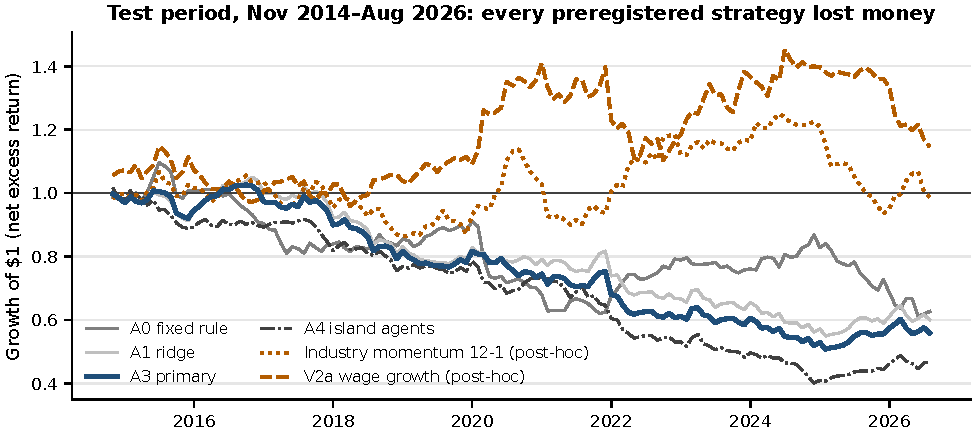
\includegraphics[width=0.9\linewidth]{figures/fig_cumulative.pdf}
\caption{Cumulative net returns in the test: every Study 1 strategy lost money; the post-hoc wage-growth book gained until 2024 and gave much of it back. Revised data for W. \hfill\tagc\ (A0--A4) / \tagp\ (momentum, W)} % src: claim C08 (A0-A4); analysis/output/study2/tables/v2_monthly_net.csv (W)
\label{fig:cumulative}
\end{figure}

\subsection*{Diagnostics of the failure}
\begin{table}[H]\centering\scriptsize\caption{Tightness regimes: months per bin under the expanding-tercile rule and under a 12-month change rule. \hfill\tagp}\setlength{\tabcolsep}{4pt}\fit{% POST-HOC | source: analysis/output/tables/d3_regime_balance.csv (generated by analysis/run.ipynb)
\begin{tabular}{lrr}
\toprule
Months in regime & Research 2004--14 & Test 2014--26 \\
\midrule
months & 125 & 142 \\
expanding low & 49 & 3 \\
expanding middle & 26 & 6 \\
expanding high & 50 & 133 \\
T rising (12m) & 93 & 88 \\
T falling (12m) & 32 & 54 \\
V/U > 1 & 0 & 75 \\
T min & $-$1.88 & $-$1.61 \\
T max & $-$0.30 & +0.71 \\
\bottomrule
\end{tabular}
}\end{table}
\begin{table}[H]\centering\scriptsize\caption{Signal IC when tightness rose or fell over the previous 12 months. \hfill\tagp}\setlength{\tabcolsep}{4pt}\fit{% POST-HOC | source: analysis/output/tables/d3_tightness_ic.csv (generated by analysis/run.ipynb)
\begin{tabular}{lrrr}
\toprule
Signal & T rising (182 m) & T falling (86 m) & Difference \\
\midrule
F1 openings & +0.001 (+0.05) & $-$0.019 ($-$0.47) & +0.019 \\
F2 hires & +0.032 (+1.51) & $-$0.026 ($-$0.74) & +0.059 \\
F3 quits & +0.024 (+1.32) & $-$0.024 ($-$0.76) & +0.048 \\
F4 layoffs & +0.013 (+0.53) & +0.060 (+1.69) & $-$0.046 \\
F5 hours & $-$0.002 ($-$0.13) & $-$0.026 ($-$1.00) & +0.024 \\
W wage growth & +0.033 (+1.67) & +0.053 (+2.04) & $-$0.020 \\
A0 composite (prereg.) & +0.003 (+0.13) & $-$0.045 ($-$1.28) & +0.048 \\
Industry momentum 12-1 & +0.036 (+1.68) & $-$0.014 ($-$0.33) & +0.050 \\
\bottomrule
\end{tabular}
}\end{table}
\begin{table}[H]\centering\footnotesize\caption{A3 profit and loss by industry in the test. \hfill\tagp}\setlength{\tabcolsep}{4pt}\fit{% POST-HOC | source: analysis/output/study1/tables/d5_industry_pnl.csv (generated by analysis/run.ipynb)
\begin{tabular}{lrrr}
\toprule
component & Contribution (pp) & Months long & Months short \\
\midrule
Mining \& logging & +7.2 & 33\% & 36\% \\
Construction & $-$19.2 & 36\% & 39\% \\
Durable mfg & +1.8 & 31\% & 24\% \\
Nondurable mfg & +5.4 & 32\% & 35\% \\
Wholesale & +14.9 & 31\% & 42\% \\
Retail & +0.2 & 39\% & 35\% \\
Transport \& utilities & +1.4 & 47\% & 30\% \\
Information & $-$5.8 & 30\% & 37\% \\
Finance \& insurance & $-$16.3 & 34\% & 45\% \\
Real estate & $-$1.6 & 24\% & 45\% \\
Prof. \& business svcs & $-$12.2 & 18\% & 47\% \\
Health care & $-$26.2 & 41\% & 36\% \\
Accommodation \& food & +4.5 & 46\% & 22\% \\
Market hedge & +4.6 &  &  \\
Trading costs & $-$13.1 &  &  \\
\bottomrule
\end{tabular}
}\end{table}
\begin{table}[H]\centering\footnotesize
\caption{Horizon profile of the A3 score against the HQ12 score, test window: rank IC ($t$ in brackets), revised data; the numbers behind \cref{fig:horizon}. \hfill\tagp}
\begin{tabular}{@{}l r r@{}}
\toprule
Horizon & A3 agent features (Study 1 primary) & HQ12 (Study 2) \\
\midrule
1 month   & $-0.021$ ($-1.08$) & $-0.020$ ($-0.87$) \\
3 months  & $-0.029$ ($-1.08$) & $+0.007$ ($+0.18$) \\
6 months  & $-0.004$ ($-0.09$) & $+0.017$ ($+0.40$) \\
9 months  & $-0.015$ ($-0.27$) & $+0.069$ ($+1.98$) \\
12 months & $-0.013$ ($-0.22$) & $+0.096$ ($+2.43$) \\
18 months & $+0.006$ ($+0.13$) & $+0.085$ ($+2.00$) \\
24 months & $-0.000$ ($-0.00$) & $+0.063$ ($+1.86$) \\
\bottomrule
\end{tabular}
\end{table}
\begin{figure}[H]
\centering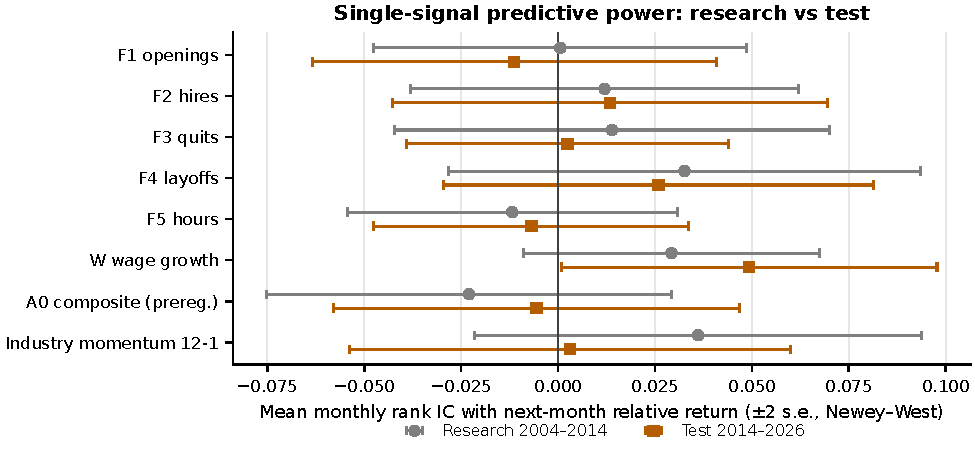
\includegraphics[width=0.9\linewidth]{figures/fig_ic_signals.pdf}
\caption{Wage growth is the only signal with a positive IC above 1.5 standard errors in both periods; layoffs and hours carry the opposite sign to the one the fixed rule imposed. \hfill\tagp} % src: d1_signal_ic.csv
\label{fig:ic_signals}
\end{figure}
\begin{figure}[H]
\centering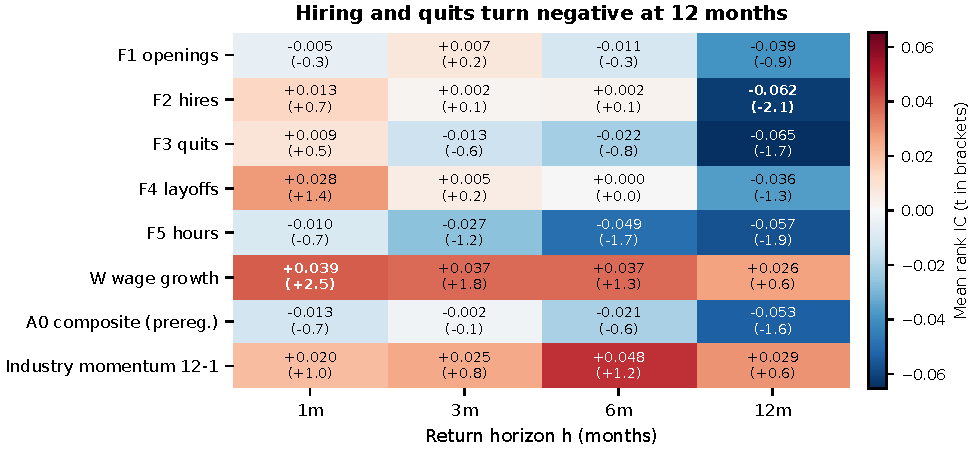
\includegraphics[width=0.86\linewidth]{figures/fig_horizon.pdf}
\caption{Hires and quits turn negative at 12 months ($t=-2.1$, $-1.7$): the investment channel shows up slowly, not within a month. \hfill\tagp} % src: claim D04
\label{fig:horizonsignals}
\end{figure}



\subsection*{The agent experiment: design and results}
The design is shown in \cref{fig:islands} of the main text; the research IC
against the test IC of every feature is in \cref{fig:agentic}.
\begin{table}[H]\centering\scriptsize\caption{Agent experiment: design parameters and counts in both studies. \hfill\tagc}\setlength{\tabcolsep}{4pt}\fit{% CONFIRMATORY | source: analysis/output/study1/tables/d10_agent_design.csv (generated by analysis/run.ipynb)
\begin{tabular}{llp{3.3in}}
\toprule
study & item & value \\
\midrule
Both & Arms & islands (communicating), independent (control) \\
Both & Agents per arm & Temporal, Composition, Interactions \\
Both & Proposals per agent x repetitions & 6 x 3 \\
Both & Migration reports & after proposals 2 and 4, at most 120 words \\
Both & Selection (repetition 1 only) & t $\geq$ 1.5, same sign in both halves, |corr| < 0.8, at most 3 per arm \\
Sonnet & Valid proposals & 98 / 108 \\
Sonnet & Migration reports admitted & 7 / 18 \\
Sonnet & Defined LLM-judge uptake labels & 8 / 36 \\
Sonnet & Human-audited judge pairs & 8 \\
Opus & Valid proposals & 106 / 108 \\
Opus & Migration reports admitted & 15 / 18 \\
Opus & Defined LLM-judge uptake labels & 84 / 88 \\
Opus & Human-audited judge pairs & 17 \\
Opus & Human-judge agreement & 10 / 17 (human yes 3, judge yes 10) \\
\bottomrule
\end{tabular}
}\end{table}
\begin{table}[H]\centering\footnotesize\caption{Agent features: how many passed the research filter and the test criterion. \hfill\tagp}\setlength{\tabcolsep}{4pt}\fit{% POST-HOC | source: analysis/output/tables/d7_agent_summary.csv (generated by analysis/run.ipynb)
\begin{tabular}{lrr}
\toprule
Repetition-1 candidates & Sonnet & Opus \\
\midrule
valid candidates & 33.0 & 35.0 \\
regime-gated & 9.0 & 6.0 \\
test IC undefined ($\leq$3 active months) & 4.0 & 2.0 \\
corr(research IC, test IC) & 0.22 & 0.37 \\
passed research filter & 4.0 & 7.0 \\
selected & 4.0 & 4.0 \\
selected and regime-gated & 2.0 & 2.0 \\
selected with positive test IC & 0.0 & 2.0 \\
\bottomrule
\end{tabular}
}\end{table}
\begin{table}[H]\centering\scriptsize\caption{Selected features, decoded after the test: research and test IC, months active. \hfill\tagp}\setlength{\tabcolsep}{4pt}\fit{% POST-HOC | source: analysis/output/study1/tables/d7_selected_features.csv (generated by analysis/run.ipynb)
\begin{tabular}{llp{2.55in}rr}
\toprule
Study & Arm & Feature (decoded) & Research IC (n) & Test IC (n) \\
\midrule
Study 1 & independent & regime(yoy(Earnings), "low") & +0.065 (48) & n/a (3) \\
Study 1 & independent & regime(spread(tsz(Layoffs, 60), tsz(Hires, 60)), "low") & +0.070 (43) & n/a (3) \\
Study 1 & communicating & spread(chg(Layoffs, 3), chg(Openings, 3)) & +0.037 (123) & $-$0.023 (142) \\
Study 1 & communicating & spread(chg(Layoffs, 6), chg(Openings, 6)) & +0.052 (120) & $-$0.004 (142) \\
Study 1b & independent & mult(regime(tsz(Hires, "exp"), "high"), csrank(tsz(Openings, "exp"))) & +0.088 (15) & $-$0.028 (133) \\
Study 1b & communicating & tsz(lchg(lag(Earnings, 1), 12), 36) & +0.064 (78) & +0.022 (142) \\
Study 1b & communicating & regime(spread(chg(Quits, 3), chg(Hires, 3)), "low") & +0.125 (48) & n/a (3) \\
Study 1b & communicating & tsz(lchg(lag(Hours, 1), 12), 36) & +0.057 (78) & +0.011 (142) \\
\bottomrule
\end{tabular}
}\end{table}

\subsection*{The agents' formula grammar}\phantomsection\label{app:grammar}
Every proposal is a formula built from the 14 operations below
(\texttt{GRAMMAR} in Study~1's \path{params.py}). The inputs are the six
anonymised variables V01 to V06 (openings, hires, quits and layoffs rates,
hours and earnings, in an order the agents never saw) and tightness $T$.

\begin{table}[H]
\centering\footnotesize
\caption{The 14 operations of the agents' grammar. \hfill\tagc}
\label{tab:grammar}
\begin{tabularx}{\textwidth}{@{}r l X@{}}
\toprule
 & Operation & What it computes \\
\midrule
1  & \texttt{lag(x,k)}     & value of $x$, $k$ months earlier ($k=1,2,3,6,12$) \\
2  & \texttt{mavg(x,w)}    & moving average of $x$ over $w$ months ($w=3,6,12$) \\
3  & \texttt{chg(x,k)}     & change: $x - \texttt{lag}(x,k)$ \\
4  & \texttt{lchg(x,k)}    & log change: $\log x - \log \texttt{lag}(x,k)$ \\
5  & \texttt{yoy(x)}       & year-over-year change: $x - \texttt{lag}(x,12)$ \\
6  & \texttt{accel(x)}     & acceleration: \texttt{chg(chg(x,3),3)} \\
7  & \texttt{persist(x,k)} & share of months with a positive one-month change over the last $k$ months ($k=3,6$) \\
8  & \texttt{tsz(x,w)}     & time-series z-score: ($x$ minus its rolling or expanding mean) over its standard deviation ($w=36$, $60$ or expanding with a 36-month minimum) \\
9  & \texttt{csrank(x)}    & cross-sectional rank: average fractional rank across the 13 groups \\
10 & \texttt{ratio(x,y)}   & $x/y$ (nonzero denominator required) \\
11 & \texttt{spread(x,y)}  & difference of cross-sectional z-scores of $x$ and $y$ \\
12 & \texttt{mult(x,y)}    & product $x\cdot y$ \\
13 & \texttt{withT(x)}     & $x$ interacted with tightness $T$ \\
14 & \texttt{regime(x,s)}  & $x$ kept only in one tightness regime ($s=$ \texttt{"low"} or \texttt{"high"}) \\
\bottomrule
\end{tabularx}
\end{table}
Every proposal must also respect five constraints: a nesting depth of at most
three; at most two variables plus $T$; logarithms only of strictly positive
values; rolling windows only with a complete history; and no arithmetic or
operation beyond the fourteen above.

\subsection*{Study 1b: exploratory follow-up with Opus}\label{app:opus}
After the test had been opened, the agent experiment was rerun with Claude
Opus~5.5 at extra-high effort, with fresh agents and the same evaluator,
selection rule and portfolio. Because the test period was already known to the
team, the run is exploratory. Its research-selected primary, A4 (agent
features, communicating), earned a test Sharpe of $+0.01$ (research $-0.40$)
with an IC of $-0.002$ ($t=-0.10$), an alpha $t$ of 0.05, a placebo $p$ of 0.56
and a Sharpe of $-0.19$ at 25\,bp; it failed gates G2 to G5 and had a Sharpe of
$-1.41$ over the last 18 months. % src: claims X01, X02
Its gross return came from one long position: durable manufacturing contributed
$+0.27$ of cumulative gross return (sum of monthly contributions, in units of
the book) in a group that is 60\% semiconductors. % src: claims X04, S03
Its A3 earned $-0.46$. % src: claim X03
The follow-up is evidence about agents, not about the strategy. A stronger model
followed the protocol better and found no more signal: 106 of 108 valid
proposals against 98, 15 of 18 admitted migration reports against 7, 84 of 88
usable judge labels against 8 of 36, % src: claims A01, A02
yet no selected feature survived the test criterion in either study. % src: claim C19

% ---------------------------------------------------------------------
\section{Study 2 in full: the post-hoc iteration}\label{app:study2}
% ---------------------------------------------------------------------
The main text reports Study~2 on data as known (Study~2.3). Studies 2.1 and 2.2
were first run on revised data with fixed publication lags; both versions are
reported below.

\subsection*{Specifications, hashes and look counts}
\begin{table}[H]
\centering\footnotesize
\caption{Every Study 2 stage was written, hashed and committed before it ran. Times are UTC. \hfill\tagp\ / \tagf}
\label{tab:specs}
\begin{tabularx}{\textwidth}{@{}l l l l X@{}}
\toprule
Specification (\texttt{analysis/specs/}) & SHA-256 & Frozen & First run & Looks counted in the deflated Sharpe \\
\midrule
\texttt{study2\_1\_variants.md} & \texttt{ca658234} & 3 Oct, 09:00:13 & 09:01:55 & 112: about 108 diagnostic looks already taken, plus the 4 variants \\ % src: claim F08
\texttt{forward\_spec.md} & \texttt{735a8ffa} & 3 Oct, 09:03:56 & book 09:17:55 & none (forward test) \\ % src: claims F08, F09
\texttt{forward\_amendment\_001.md} & \texttt{c76cde86} & 3 Oct, 09:16:11 & book 09:17:55 & none \\ % src: claim F08
\texttt{study2\_2\_hq12\_robustness.md} & \texttt{312aef1d} & 3 Oct, 09:52:27 & 09:53:32 & 132: 112 plus 20 battery backtests \\ % src: claim F08
\texttt{study2\_3\_robustness.md} & \texttt{068a3e03} & 4 Oct, 09:18:39 & 09:26:27 & 162: 132 plus 30 (24 as-known, 4 cap, 2 rank-weighted) \\ % src: claim T25
\bottomrule
\end{tabularx}
\end{table}
The run logs (\path{analysis/output/study2/v2_run_log.md},
\path{v3_run_log.md}, \path{study2_3_run_log.md}) hold the SHA-256 of every
result table at its first run; the notebook recomputes them on each run and
stops if one differs. Result files of Studies 2.1 and 2.2 keep the codes V2a to
V2d inside (\cref{app:names}).

\subsection*{Study 2.1: the four variants}
\begin{table}[H]
\centering\footnotesize
\caption{Post-hoc variants on revised data: net Sharpe by window and test statistics at 10\,bp. Test figures are the test slice of a continuous run from May 2004 (A3's ledger starts from an empty book in November 2014). IC, alpha $t$ and placebo are one-month statistics with 6 Newey--West lags; DSR counts 112 looks as independent trials, a rough deflation since the looks are correlated. \hfill\tagp} % src: analysis/specs/study2_1_variants.md section 5
\label{tab:v2}
\fit{% POST-HOC | source: analysis/output/tables/v2_results.csv (generated by analysis/run.ipynb)
\begin{tabular}{lrrrrrrrrr}
\toprule
Variant & Research & Test & Full & Post-2010 & Last 18m & Test IC (t) & Alpha t & Placebo p & DSR \\
\midrule
V2a & +0.09 & +0.16 & +0.15 & +0.12 & $-$1.71 & +0.049 (+2.04) & +0.29 & 0.02 & 0.02 \\
V2b & $-$0.06 & $-$0.15 & $-$0.11 & $-$0.16 & $-$1.34 & +0.042 (+1.65) & $-$0.84 & 0.05 & 0.00 \\
V2c & +0.27 & +0.35 & +0.32 & +0.24 & $-$0.78 & +0.032 (+1.21) & +1.36 & 0.26 & 0.09 \\
V2d & +0.50 & +0.29 & +0.35 & +0.30 & +0.29 & $-$0.020 ($-$0.87) & +1.37 & 0.85 & 0.06 \\
\bottomrule
\end{tabular}
}
\end{table}
The reading rule declared with the variants: positive Sharpe at 25\,bp, IC
$t\ge2$, alpha $t\ge2$, positive IC in both test halves, placebo $p<0.05$ and
DSR above 0.95; none of the four meets it. % src: claim V07
HQ12's pre-declared one-month placebo $p$ is 0.85; a horizon-matched placebo
added after the run gives 0.06 in the test and 0.04 over the full sample. % src: claim V09


\subsection*{Study 2.2: the HQ12 battery on revised data}
\begin{figure}[H]
\centering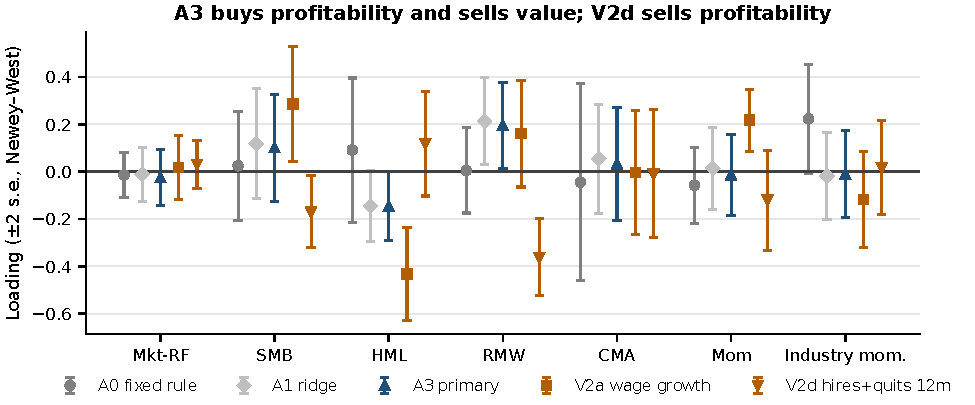
\includegraphics[width=0.9\linewidth]{figures/fig_loadings.pdf}
\caption{Factor loadings of the long--short books (\cref{sec:style}): A3 buys profitability and sells value; HQ12 sells profitability. \hfill\tagc\ (A0, A1, A3) / \tagp\ (W, HQ12)}
\label{fig:loadings}
\end{figure}

\begin{table}[H]\centering\footnotesize\caption{R3 holding period: Sharpe by window. \hfill\tagp}\setlength{\tabcolsep}{4pt}\fit{% POST-HOC | source: analysis/output/study2/tables/v3_r3_holding.csv (generated by analysis/run.ipynb)
\begin{tabular}{lrrrrrr}
\toprule
Holding & research & test & full & post-2010 & last 18m & Test turnover \\
\midrule
6 months & +0.31 & +0.05 & +0.15 & +0.05 & +0.50 & 0.49 \\
9 months & +0.43 & +0.14 & +0.24 & +0.16 & +0.29 & 0.40 \\
12 months & +0.50 & +0.29 & +0.35 & +0.30 & +0.29 & 0.37 \\
18 months & +0.58 & +0.30 & +0.38 & +0.34 & +0.31 & 0.28 \\
\bottomrule
\end{tabular}
}\end{table}
\begin{table}[H]\centering\footnotesize\caption{R4 sub-periods. \hfill\tagp}\setlength{\tabcolsep}{4pt}\fit{% POST-HOC | source: analysis/output/tables/v3_r4_subperiods.csv (generated by analysis/run.ipynb)
\begin{tabular}{lrrrr}
\toprule
Window & Months & Sharpe & Net p.a. & IC 12m (t) \\
\midrule
test: first half & 71 & $-$0.21 & $-$1.4\% & +0.097 (+1.75) \\
test: second half & 71 & +0.64 & +6.5\% & +0.095 (+1.60) \\
test: excl. Mar 2020-Dec 2021 & 120 & +0.37 & +3.0\% & +0.105 (+2.23) \\
test: pre-2020 & 62 & +0.14 & +0.8\% & +0.114 (+1.92) \\
test: 2020 onward & 80 & +0.37 & +3.9\% & +0.080 (+1.54) \\
full: first half & 134 & +0.33 & +2.0\% & +0.038 (+0.73) \\
full: second half & 134 & +0.38 & +3.3\% & +0.107 (+2.66) \\
full: excl. Mar 2020-Dec 2021 & 246 & +0.40 & +2.9\% & +0.073 (+1.93) \\
full: pre-2020 & 188 & +0.36 & +2.2\% & +0.068 (+1.57) \\
\bottomrule
\end{tabular}
}\end{table}
\begin{table}[H]\centering\footnotesize\caption{R5 costs: Sharpe by cost level and break-even. \hfill\tagp}\setlength{\tabcolsep}{4pt}\fit{% POST-HOC | source: analysis/output/study2/tables/v3_r5_costs.csv (generated by analysis/run.ipynb)
\begin{tabular}{lrrrrr}
\toprule
Window & 0 bp & 10 bp & 25 bp & 50 bp & Break-even (bp) \\
\midrule
research & +0.58 & +0.50 & +0.39 & +0.20 & 76 \\
test & +0.34 & +0.29 & +0.22 & +0.09 & 68 \\
full & +0.41 & +0.35 & +0.26 & +0.11 & 69 \\
post-2010 & +0.35 & +0.30 & +0.21 & +0.07 & 63 \\
last 18m & +0.32 & +0.29 & +0.24 & +0.16 & 99 \\
\bottomrule
\end{tabular}
}\end{table}
\begin{table}[H]\centering\footnotesize
\caption{R6 factor regression of HQ12 with 12 Newey--West lags, revised data: loadings ($t$ in brackets). \hfill\tagp}
\begin{tabular}{@{}l r r@{}}
\toprule
 & Test & Full sample \\
\midrule
Alpha (per month)  & $+0.26\%$ ($+1.48$) & $+0.26\%$ ($+1.92$) \\
Market             & $+0.03$ ($+0.58$)   & $-0.00$ ($-0.08$) \\
SMB                & $-0.17$ ($-2.24$)   & $-0.02$ ($-0.31$) \\
HML                & $+0.12$ ($+1.07$)   & $+0.10$ ($+1.23$) \\
RMW                & $-0.36$ ($-4.45$)   & $-0.16$ ($-1.83$) \\
CMA                & $-0.01$ ($-0.07$)   & $-0.09$ ($-0.87$) \\
Momentum           & $-0.12$ ($-1.14$)   & $-0.03$ ($-0.51$) \\
Industry momentum  & $+0.02$ ($+0.17$)   & $+0.06$ ($+0.93$) \\
\bottomrule
\end{tabular}
\end{table}
\begin{table}[H]\centering\footnotesize\caption{R7 drop one group, every run. \hfill\tagp}\setlength{\tabcolsep}{4pt}\fit{% POST-HOC | source: analysis/output/study2/tables/v3_r7_dropone.csv (generated by analysis/run.ipynb)
\begin{tabular}{lrrr}
\toprule
industry & dropped group & test sharpe & full sharpe \\
\midrule
Mining \& logging & 1 & +0.33 & +0.25 \\
Construction & 2 & +0.30 & +0.34 \\
Durable mfg & 3 & +0.30 & +0.30 \\
Nondurable mfg & 4 & +0.40 & +0.36 \\
Wholesale & 5 & +0.36 & +0.37 \\
Retail & 6 & +0.29 & +0.35 \\
Transport \& utilities & 7 & +0.30 & +0.34 \\
Information & 8 & +0.41 & +0.54 \\
Finance \& insurance & 9 & +0.23 & +0.23 \\
Real estate & 10 & +0.48 & +0.43 \\
Prof. \& business svcs & 11 & +0.26 & +0.33 \\
Health care & 12 & +0.18 & +0.36 \\
Accommodation \& food & 13 & +0.32 & +0.28 \\
\bottomrule
\end{tabular}
}\end{table}
\begin{table}[H]\centering\footnotesize\caption{R9 block-bootstrap 90\% interval. \hfill\tagp}\setlength{\tabcolsep}{4pt}\fit{% POST-HOC | source: analysis/output/tables/v3_r9_bootstrap.csv (generated by analysis/run.ipynb)
\begin{tabular}{lrrrr}
\toprule
Window & Sharpe & 90\% interval & Months & Excludes 0 \\
\midrule
test & +0.29 & [$-$0.07, +0.65] & 142 & no \\
full & +0.35 & [+0.05, +0.64] & 268 & yes \\
\bottomrule
\end{tabular}
}\end{table}
\begin{table}[H]\centering\footnotesize\caption{R11 fundamental law in the test window: IC, breadth, transfer coefficient, implied and realised ratio, revised data. \hfill\tagc\ (A3) / \tagp}\setlength{\tabcolsep}{4pt}\fit{% CONFIRMATORY (A3) / POST-HOC | source: analysis/output/tables/v3_r11_fundamental_law.csv (generated by analysis/run.ipynb)
\begin{tabular}{lrrrrrrr}
\toprule
Book (test window) & IC & Horizon & BR/yr & TC & Implied IR & Ceiling (TC=1) & Realised Sharpe \\
\midrule
A3 primary & $-$0.021 & 1m & 156 & 0.80 & $-$0.21 & $-$0.27 & $-$0.58 \\
V2a wage growth & +0.049 & 1m & 156 & 0.91 & +0.56 & +0.62 & +0.16 \\
V2d -(hires+quits) 12m & +0.096 & 12m & 13 & 0.48 & +0.17 & +0.35 & +0.29 \\
\bottomrule
\end{tabular}
}\end{table}
\begin{table}[H]\centering\footnotesize\caption{The pre-declared reading of the battery on revised data: HQ12 is fragile on R4. \hfill\tagp}\setlength{\tabcolsep}{4pt}\fit{% POST-HOC | source: analysis/output/tables/v3_reading.csv (generated by analysis/run.ipynb)
\begin{tabular}{lr}
\toprule
condition & holds \\
\midrule
R1 hires-only and quits-only test Sharpe > 0 & yes \\
R2 test 12m IC t >= 2 and 1m IC t < 2 & yes \\
R3 holding 9 and 18 months test Sharpe > 0 & yes \\
R4 both test halves Sharpe > 0 & no \\
R5 test break-even cost > 25 bp & yes \\
R7 minimum drop-one test Sharpe > 0 & yes \\
R9 90\% interval excludes 0 (test or full) & yes \\
\bottomrule
\end{tabular}
}\end{table}
\begin{figure}[H]
\centering
\begin{subfigure}[t]{0.48\linewidth}\centering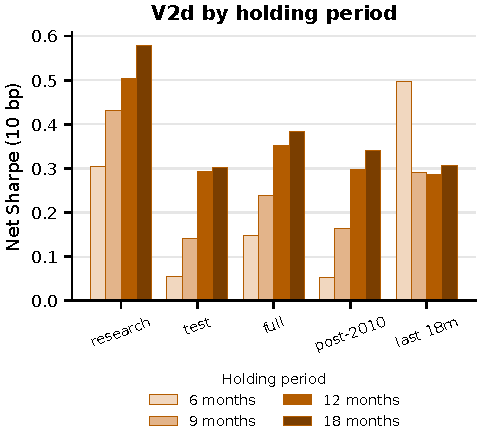
\includegraphics[width=\linewidth]{figures/fig_v2d_holding.pdf}\end{subfigure}\hfill
\begin{subfigure}[t]{0.48\linewidth}\centering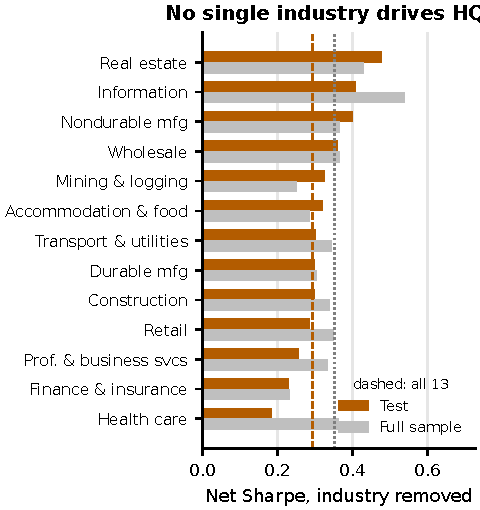
\includegraphics[width=\linewidth]{figures/fig_v2d_dropone.pdf}\end{subfigure}
\caption{Left: HQ12 is positive at every holding period from 6 to 18 months. Right: no single industry carries HQ12; removing any one leaves its test Sharpe between $+0.18$ and $+0.48$ on revised data ($+0.05$ and $+0.36$ as known). \hfill\tagp} % src: claims R3a, R7a
\label{fig:v2d_holding}
\end{figure}
\begin{figure}[H]
\centering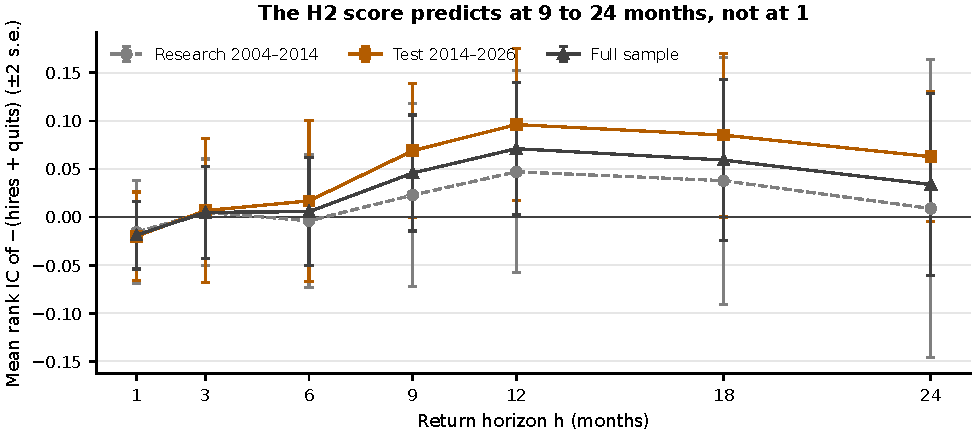
\includegraphics[width=0.6\linewidth]{figures/fig_horizon_profile.pdf}
\caption{Horizon profile of the HQ12 score in every window: no one-month IC, positive from 9 to 24 months. \hfill\tagp} % src: claim R2a
\label{fig:horizon_profile}
\end{figure}


\subsection*{Study 2.3: as-known rerun, risk overlay, rank weights, agents, capacity}
The as-known inputs come from Alex's data package. Before any variant was rerun
we rebuilt his raw features from the as-known panel and his A0 score from his
standardised features: both match his saved files to machine precision. % src: claim T01
\begin{table}[H]\centering\footnotesize\caption{R1: the four variants on fixed-lag and on as-known data, test window. The last two columns are the share of months in which both versions rank the same three groups highest and lowest. \hfill\tagp}\setlength{\tabcolsep}{4pt}\fit{% POST-HOC | source: analysis/output/study2/tables/s23_r1_variants.csv (generated by analysis/run.ipynb)
\begin{tabular}{lrrrrrrr}
\toprule
Variant (test window) & Sharpe, fixed lag & Sharpe, as known & IC (t), fixed lag & IC (t), as known & Alpha t & Same top 3 & Same bottom 3 \\
\midrule
W & +0.16 & +0.13 & +0.049 (+2.04) & +0.041 (+1.73) & +0.18 & 76\% & 70\% \\
SC & $-$0.15 & +0.24 & +0.042 (+1.65) & +0.021 (+0.75) & +0.71 & 0\% & 0\% \\
W+MOM & +0.35 & +0.46 & +0.032 (+1.21) & +0.036 (+1.40) & +1.93 & 84\% & 74\% \\
HQ12 & +0.29 & +0.20 & +0.096 (+2.43) & +0.085 (+2.26) & +0.92 & 39\% & 51\% \\
\bottomrule
\end{tabular}
}\end{table} % src: claims T02, T03, T04
\begin{table}[H]\centering\footnotesize\caption{R1: HQ12 battery, fixed lag against as known, every row; the source of \cref{tab:battery}. \hfill\tagp}\setlength{\tabcolsep}{4pt}\fit{% POST-HOC | source: analysis/output/study2/tables/s23_r1_hq12_battery.csv (generated by analysis/run.ipynb)
\begin{tabular}{lrr}
\toprule
HQ12 check & Fixed lag (Study 2.2) & As known (Study 2.3) \\
\midrule
Test Sharpe (10 bp) & +0.29 & +0.20 \\
Full-sample Sharpe (10 bp) & +0.35 & +0.31 \\
12-month IC, test & +0.10 & +0.08 \\
12-month IC t, test & +2.43 & +2.26 \\
1-month IC t, test & $-$0.87 & $-$0.42 \\
Component hires only, test Sharpe & +0.19 & +0.19 \\
Component quits only, test Sharpe & +0.16 & +0.17 \\
Holding 9 months, test Sharpe & +0.14 & +0.16 \\
Holding 18 months, test Sharpe & +0.30 & +0.11 \\
First test half, Sharpe & $-$0.21 & $-$0.23 \\
Second test half, Sharpe & +0.64 & +0.49 \\
Test Sharpe at 0 bp & +0.34 & +0.25 \\
Test Sharpe at 25 bp & +0.22 & +0.13 \\
Test Sharpe at 50 bp & +0.09 & $-$0.00 \\
Break-even cost, test (bp) & 68 & 50 \\
Drop one group, minimum test Sharpe & +0.18 & +0.05 \\
Drop one group, maximum test Sharpe & +0.48 & +0.36 \\
Bootstrap 90\% interval, test: low & $-$0.07 & $-$0.14 \\
Bootstrap 90\% interval, test: high & +0.65 & +0.57 \\
Alpha per month (\%), test, HAC 12 & +0.26 & +0.16 \\
Alpha t, test, HAC 12 & +1.48 & +0.92 \\
Bootstrap 90\% interval, full: low & +0.05 & +0.02 \\
Bootstrap 90\% interval, full: high & +0.64 & +0.60 \\
Alpha per month (\%), full, HAC 12 & +0.26 & +0.21 \\
Alpha t, full, HAC 12 & +1.92 & +1.81 \\
Deflated Sharpe, test (132 looks fixed lag; 162 as known) & +0.05 & +0.02 \\
\bottomrule
\end{tabular}
}\end{table}
\begin{table}[H]\centering\footnotesize\caption{R2: ex-ante volatility of the unit book and gross exposure needed to reach 10\%: 5th, 50th and 95th percentile over the test months. \hfill\tagp}\setlength{\tabcolsep}{4pt}\fit{% POST-HOC | source: analysis/output/study2/tables/s23_r2_distribution.csv (generated by analysis/run.ipynb)
\begin{tabular}{lrrrrrr}
\toprule
book & unit vol p5 & unit vol p50 & unit vol p95 & gross needed p5 & gross needed p50 & gross needed p95 \\
\midrule
A3 & 0.045 & 0.075 & 0.110 & 1.85 & 2.60 & 4.19 \\
HQ12 & 0.033 & 0.064 & 0.103 & 1.79 & 2.45 & 4.24 \\
\bottomrule
\end{tabular}
}\end{table}
\begin{table}[H]\centering\footnotesize\caption{R3: top 3 / bottom 3 against rank-weighted books, test window. TC is the transfer coefficient; the implied IR is IC $\times\sqrt{\text{BR}}\times$ TC. \hfill\tagp}\setlength{\tabcolsep}{4pt}\fit{% POST-HOC | source: analysis/output/study2/tables/s23_r3_rank_weighted.csv (generated by analysis/run.ipynb)
\begin{tabular}{llrrrr}
\toprule
Book & Weights & Test Sharpe & TC & Turnover & Implied IR \\
\midrule
A3 & top 3 / bottom 3 & $-$0.58 & 0.80 & 0.91 & $-$0.21 \\
A3 & rank-weighted & $-$0.49 & 0.83 & 0.86 & $-$0.22 \\
HQ12 & top 3 / bottom 3 & +0.29 & 0.48 & 0.37 & +0.17 \\
HQ12 & rank-weighted & +0.31 & 0.49 & 0.37 & +0.17 \\
\bottomrule
\end{tabular}
}\end{table}
\begin{table}[H]\centering\footnotesize\caption{Turnover and costs in the test window, revised data. Break-even is the industry cost at which the net return is zero. \hfill\tagc\ (A3) / \tagp}\setlength{\tabcolsep}{4pt}\fit{% CONFIRMATORY (A3) / POST-HOC | source: analysis/output/study2/tables/s23_costs_turnover.csv (generated by analysis/run.ipynb)
\begin{tabular}{lrrrrr}
\toprule
Book (test window) & Turnover p.a. & Cost drag p.a. & Gross p.a. & Net p.a. & Break-even (bp) \\
\midrule
A3 agent features, independent (primary) & 11.0x & 1.11\% & $-$3.5\% & $-$4.6\% & $-$32 \\
W wage growth (declared headline) & 4.7x & 0.47\% & +2.1\% & +1.7\% & +46 \\
SC signed composite & 8.7x & 0.88\% & $-$0.5\% & $-$1.3\% & $-$5 \\
W+MOM wage growth + momentum & 5.8x & 0.59\% & +3.6\% & +3.1\% & +62 \\
HQ12 hires + quits reversal, 12-month hold & 4.4x & 0.44\% & +3.0\% & +2.6\% & +68 \\
A3 rank-weighted & 10.3x & 1.05\% & $-$2.5\% & $-$3.6\% & $-$24 \\
HQ12 rank-weighted & 4.4x & 0.45\% & +3.0\% & +2.6\% & +69 \\
\bottomrule
\end{tabular}
}\end{table}
\begin{table}[H]\centering\footnotesize\caption{R4: agent proposals by study, arm and seed: valid proposals, best and mean research IC, eligible features (seed 1 only) and share with a regime gate. \hfill\tagp}\setlength{\tabcolsep}{4pt}\fit{% POST-HOC | source: analysis/output/study2/tables/s23_r4_agents_by_seed.csv (generated by analysis/run.ipynb)
\begin{tabular}{llrrrrrr}
\toprule
Study & Arm & Seed & Valid & Best IC & Mean IC & Eligible & Regime-gated \\
\midrule
Study 1 & independent & 1 & 17/18 & +0.101 & +0.014 & 2 & 29\% \\
Study 1 & independent & 2 & 17/18 & +0.102 & $-$0.006 &  & 24\% \\
Study 1 & independent & 3 & 13/18 & +0.046 & $-$0.014 &  & 15\% \\
Study 1 & communicating & 1 & 16/18 & +0.052 & $-$0.003 & 2 & 25\% \\
Study 1 & communicating & 2 & 17/18 & +0.058 & +0.005 &  & 6\% \\
Study 1 & communicating & 3 & 18/18 & +0.037 & $-$0.008 &  & 22\% \\
Study 1b & independent & 1 & 18/18 & +0.088 & $-$0.002 & 1 & 28\% \\
Study 1b & independent & 2 & 18/18 & +0.045 & $-$0.006 &  & 11\% \\
Study 1b & independent & 3 & 18/18 & +0.045 & +0.002 &  & 6\% \\
Study 1b & communicating & 1 & 17/18 & +0.125 & +0.026 & 6 & 6\% \\
Study 1b & communicating & 2 & 18/18 & +0.191 & +0.049 &  & 39\% \\
Study 1b & communicating & 3 & 17/18 & +0.091 & +0.009 &  & 47\% \\
\bottomrule
\end{tabular}
}\end{table}
\begin{table}[H]\centering\scriptsize\caption{R4: arm gap against seed spread, exact permutation test over 20 relabelings. \hfill\tagp}\setlength{\tabcolsep}{4pt}\fit{% POST-HOC | source: analysis/output/study2/tables/s23_r4_permutation.csv (generated by analysis/run.ipynb)
\begin{tabular}{lrrrrrr}
\toprule
study & metric & islands minus independent & largest seed range within arm & gap within seed range & perm p two sided & relabelings \\
\midrule
Study 1 (Sonnet) & best\_ic & $-$0.034 & 0.056 & True & 0.30 & 20 \\
Study 1 (Sonnet) & mean\_ic & $-$0.001 & 0.028 & True & 1.00 & 20 \\
Study 1b (Opus) & best\_ic & +0.076 & 0.099 & True & 0.10 & 20 \\
Study 1b (Opus) & mean\_ic & +0.030 & 0.040 & True & 0.10 & 20 \\
\bottomrule
\end{tabular}
}\end{table}
\begin{table}[H]\centering\footnotesize\caption{R5: tokens per proposal call by arm. \hfill\tagp}\setlength{\tabcolsep}{4pt}\fit{% POST-HOC | source: analysis/output/study2/tables/s23_r5_tokens.csv (generated by analysis/run.ipynb)
\begin{tabular}{llrrrr}
\toprule
Study & Arm & Calls & Tokens, total & Tokens per call & Output tokens per call \\
\midrule
Study 1 & independent & 54 & 120,932 & 2,239 & 183 \\
Study 1 & communicating & 54 & 134,185 & 2,485 & 193 \\
Study 1b & independent & 54 & 180,555 & 3,344 & 1,257 \\
Study 1b & communicating & 54 & 214,003 & 3,963 & 1,509 \\
\bottomrule
\end{tabular}
}\end{table}
\begin{table}[H]\centering\footnotesize\caption{R5: Spearman correlation between a proposal's output tokens and its research IC. \hfill\tagp}\setlength{\tabcolsep}{4pt}\fit{% POST-HOC | source: analysis/output/study2/tables/s23_r5_tokens_ic.csv (generated by analysis/run.ipynb)
\begin{tabular}{lrrr}
\toprule
study & n & spearman output tokens vs ic & spearman output tokens vs abs ic \\
\midrule
Study 1 (Sonnet) & 98 & +0.13 & +0.21 \\
Study 1b (Opus) & 106 & +0.41 & +0.24 \\
\bottomrule
\end{tabular}
}\end{table}
\begin{table}[H]\centering\footnotesize\caption{R6: participation ratio of the 13-group correlation matrices. \hfill\tagp}\setlength{\tabcolsep}{4pt}\fit{% POST-HOC | source: analysis/output/study2/tables/s23_r6_breadth.csv (generated by analysis/run.ipynb)
\begin{tabular}{lr}
\toprule
matrix & participation\_ratio \\
\midrule
13 group excess returns & 2.0 \\
13 group relative returns (group minus equal-weight mean) & 9.1 \\
z(W) across groups & 7.4 \\
HQ12 score across groups & 10.1 \\
\bottomrule
\end{tabular}
}\end{table}
\begin{table}[H]\centering\scriptsize\caption{R7: capacity with the proxy ETFs: the binding ETF, its average daily dollar volume, and the assets at which monthly trading reaches 1\% and 5\% of it. \hfill\tagp}\setlength{\tabcolsep}{4pt}\fit{% POST-HOC | source: analysis/output/study2/tables/s23_r7_capacity.csv (generated by analysis/run.ipynb)
\begin{tabular}{lrrrrrrrr}
\toprule
book & binding\_etf & binding\_adv\_usd\_m & monthly\_trade\_share\_of\_aum & aum\_at\_1pct\_adv\_usd\_m & aum\_at\_5pct\_adv\_usd\_m & spy\_adv\_usd\_bn & smallest\_etf\_adv\_usd\_m & smallest\_etf \\
\midrule
A3 & PEJ & 3.2 & 0.063 & 0.5 & 2.5 & 47.0 & 3.2 & PEJ \\
HQ12 & PEJ & 3.2 & 0.027 & 1.2 & 5.9 & 47.0 & 3.2 & PEJ \\
\bottomrule
\end{tabular}
}\end{table}
\begin{table}[H]\centering\scriptsize\caption{R8: judge with a verbatim quote on the 25 hand-labelled pairs. ``Usable'' counts JSON-only answers; the third row of each study accepts JSON wrapped in a code fence and is outside the pre-declared rule. \hfill\tagp}\setlength{\tabcolsep}{4pt}\fit{% POST-HOC | source: analysis/output/study2/tables/s23_r8_judge_summary.csv (generated by analysis/run.ipynb)
\begin{tabular}{lrrrrrrrr}
\toprule
study & judge & pairs & defined & agree & judge\_yes & human\_yes & false\_yes & missed\_yes \\
\midrule
Study 1 (Sonnet) & original judge & 8 & 2 & 1 & 1 & 1 & 1 & 0 \\
Study 1 (Sonnet) & judge with verbatim quote & 8 & 8 & 7 & 2 & 1 & 1 & 0 \\
Study 1 (Sonnet) & with quote, fenced JSON accepted (supplementary) & 8 & 8 & 7 & 2 & 1 & 1 & 0 \\
Study 1b (Opus) & original judge & 17 & 17 & 10 & 10 & 3 & 7 & 0 \\
Study 1b (Opus) & judge with verbatim quote & 17 & 7 & 3 & 5 & 3 & 4 & 0 \\
Study 1b (Opus) & with quote, fenced JSON accepted (supplementary) & 17 & 17 & 9 & 11 & 3 & 8 & 0 \\
\bottomrule
\end{tabular}
}\end{table}
\begin{table}[H]\centering\scriptsize\caption{R9: feedback ablation, independent arm, research data only, with and without the tightness-tercile split in the feedback. ``Informative'' counts months in which a proposal's cross-section is not constant. \hfill\tagp}\label{tab:r9}\setlength{\tabcolsep}{4pt}\fit{% POST-HOC | source: analysis/output/study2/tables/s23_r9_ablation_summary.csv (generated by analysis/run.ipynb)
\begin{tabular}{lrrrrrrr}
\toprule
Feedback & Seeds & Proposals & Valid & With a regime gate & Share & Informative in under half of months & Best research IC \\
\midrule
with tercile split & 3 & 54 & 48 & 4 & 8\% & 8\% & +0.070 \\
without tercile split & 3 & 54 & 50 & 3 & 6\% & 6\% & +0.070 \\
\bottomrule
\end{tabular}
}\end{table}
The ablation rebuilt the agents' research inputs from Alex's package; they
reproduce 94 of the 98 saved feedbacks exactly, and the largest difference is
0.11 in a $t$-statistic. % src: claim T21
The judge calls for Study~1b pairs used a newer command-line client than the
Study~1 pairs because the older one does not serve that model; calls that
failed in transport were repeated once, and every call is in the log
(\path{analysis/output/study2/llm/}).
\begin{figure}[H]
\centering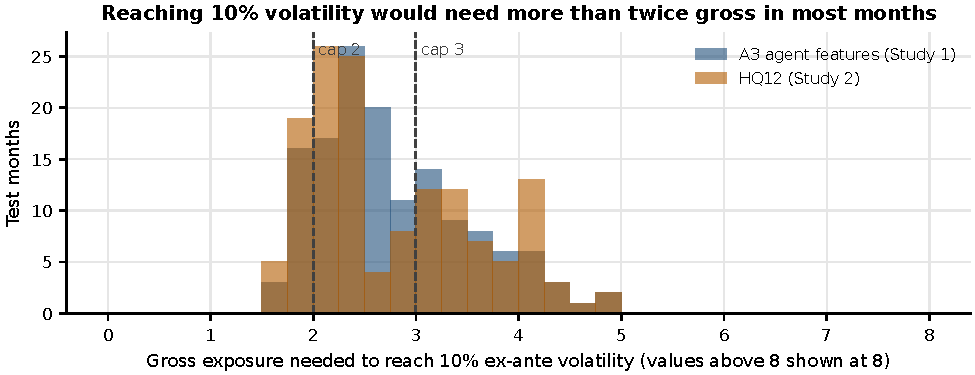
\includegraphics[width=0.8\linewidth]{figures/fig_s23_gross_needed.pdf}
\caption{Reaching 10\% volatility would need more than twice gross in most test months, so the cap of 2 binds. \hfill\tagp} % src: claim T10
\label{fig:gross}
\end{figure}
\begin{figure}[H]
\centering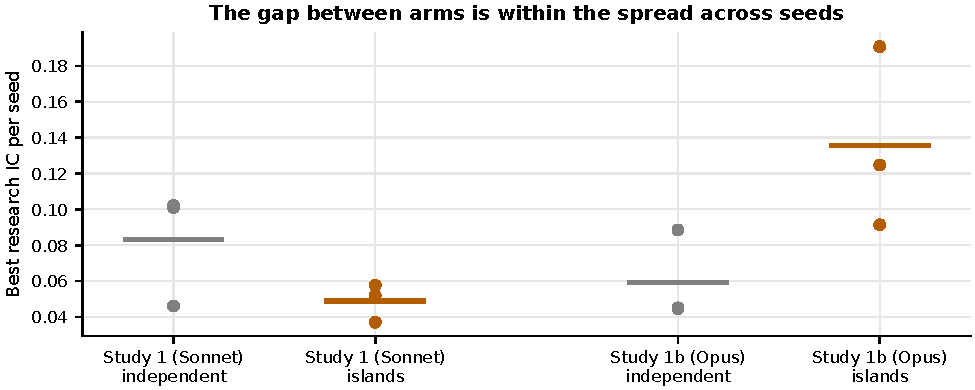
\includegraphics[width=0.8\linewidth]{figures/fig_s23_agents_seeds.pdf}
\caption{Best research IC per seed: the gap between arms is within the spread across seeds in both studies (\cref{sec:ai}). \hfill\tagp} % src: claim T13
\label{fig:seeds}
\end{figure}

% ---------------------------------------------------------------------
\section{Forward test: frozen specification and Q4 2026 books}\label{app:forward}
% ---------------------------------------------------------------------
\begin{itemize}
  \item \path{analysis/specs/study2_1_variants.md}: four post-hoc variants and a reading rule; SHA-256 \texttt{ca658234\ldots}, frozen 2026-10-03T09:00:13Z, first run 09:01:55Z. % src: claim F08
  \item \path{analysis/specs/forward_spec.md}: decision 30 September 2026, information cutoff 29 September, one tranche held to 31 December, 60-month beta hedge in SPY, 10\,bp and 2\,bp costs; SHA-256 \texttt{735a8ffa\ldots}, frozen 09:03:56Z. % src: claims F08, F05
  \item \path{analysis/specs/forward_amendment_001.md}: the fixed-lag information set (JOLTS July 2026, CES August 2026, as published on 29 September) after the pre-committed check stopped the first run; W+MOM and HQ12 added after the Study 2.1 results were seen and before any Q4 return beyond 1--2 October; SHA-256 \texttt{c76cde86\ldots}, frozen 09:16:11Z; book built 09:17:55Z. % src: claims F08, F05
  \item \path{analysis/specs/study2_2_hq12_robustness.md}: the HQ12 battery; SHA-256 \texttt{312aef1d\ldots}, frozen 09:52:27Z, first run 09:53:32Z. \path{analysis/specs/study2_3_robustness.md}: SHA-256 \texttt{068a3e03\ldots}, frozen 4 October 09:18:39Z, before its first output. % src: claims F08, T25
  \item Books: \path{analysis/output/forward/book_2026Q4.csv} (group weights for W, SC, W+MOM and HQ12), \path{book_2026Q4_etf.csv} (netted ETF weights), \path{book_2026Q4_hedge.csv} (SPY hedge per unit: $-0.40$, $-0.06$, $-0.24$, $-0.02$), \path{etf_proxies.csv}. % src: claim F03
  Holdings: W is long construction, durable manufacturing and information and short mining, health care and accommodation; % src: claim F01
  SC is long durable manufacturing, retail and transport and short real estate, health care and accommodation; W+MOM is long construction, durable manufacturing and finance and short retail, transport and professional services; % src: claims F06, F07
  HQ12 is long finance, real estate and accommodation and short mining, durable manufacturing and retail. % src: claim F02
  W+MOM's tradable book has four legs, because its long durable-manufacturing and short professional-services positions both map to the industrials ETF and cancel. % src: claim F04
  \item Power: HQ12's test volatility is about 9\% a year, so one quarter's return has a standard deviation near 5\%; a Q4 return between $-10\%$ and $+10\%$ is within two standard deviations of zero. % src: claim V04
  The book was first built at 09:17:55Z on 3 October: commit \texttt{3e8ecd7} (09:18:29Z) holds a byte-identical \path{book_2026Q4.csv} (SHA-256 \texttt{857275\ldots}); \path{book_first_build.sha256} records that first build and later notebook runs must reproduce it. % src: claim F09
  \item Horizon: HQ12 predicts returns nine to 24 months ahead and has no IC at three months, so its Q4 return will mostly measure noise. The informative evaluation is the twelve-month return of the same tranche, to 30 September 2027 (\cref{sec:robust}).
  \item Evaluation: the ETF books from the 30 September close to the 31 December close after costs, and the same books on Ken French group returns once published; reported whatever they show. Cadence: a weekly tracker was considered and deferred by team decision, since with one quarter of data and no capital at risk a weekly readout adds noise without adding power (\cref{sec:robust}). We will evaluate once at the 31 December close.
\end{itemize}

% ---------------------------------------------------------------------
\section{Claude, interaction by interaction}\label{app:claude}
% ---------------------------------------------------------------------
Condensed from the team's written evaluation. Paths are relative to \path{study1_preregistered/outputs/follow_the_workers/}
unless stated; Study~1b has the same files under
\path{follow_the_workers_opus55_xhigh/}.

Claude took every AI role: Sonnet~5.5 for Study~1, Opus~5.5 at extra-high
effort for Study~1b, and later Claude models for the post-mortem and the
iteration. This term's course allows it; the switch from the ChatGPT template is
logged as preregistration amendments 001 and 002
(\path{outputs/prereg_amendments/}, \path{outputs/deviations.md}), and the log
file keeps the template name \path{chatgpt_log.md} with Claude content. % src: claim A06

\begin{table}[H]
\centering
\caption{Claude, interaction by interaction: what it got right, what it got wrong, what we did. The detail of each interaction and the transcripts follow the table.}
\label{tab:log}
\footnotesize
\begin{tabularx}{\linewidth}{@{}>{\raggedright\arraybackslash}p{0.15\linewidth}
  >{\raggedright\arraybackslash}X >{\raggedright\arraybackslash}X
  >{\raggedright\arraybackslash}X@{}}
\toprule
Interaction & What it got right & What it got wrong & What we did \\
\midrule
P1 audit (Sonnet) & Flagged every real gap in the mapping & 5 of 25 findings unsupported; design choices called ``confirmed errors'' & Tested all 25; one metadata fix \\
P2 agents (Sonnet; Opus in 1b) & Blind protocol followed; 98 and 106 of 108 proposals valid & No feature survived the test; A3's two features active in 3 months & Mechanical selection; no proposal edited \\
P3 judge & Never missed a true reuse & 7 false yeses in 17 audited pairs & Hand audit; quote requirement tested in Study~2.3 \\
P4 red team (Sonnet) & 6 of 10 concerns matched registered tests & A $p$-value never computed; new thresholds after seeing results & Registered tests kept; new thresholds rejected \\
P5 post-mortem\ph & Traced the failure to features active in 3 months & Fixes read off the test results & Became Study~2, labelled post hoc \\
P6 iteration\ph & Reproduced Study~1 exactly; froze every stage & Wrong assumption on a JOLTS release date & Its own check stopped the run; amendment disclosed \\
\bottomrule
\end{tabularx}
\end{table}

\paragraph{P1, data and code audit} The system prompt made Claude ``a careful
data and code auditor'' with no tools; the prompt in \cref{sec:impl} was
followed by the manifest, the crosswalk and the as-of code (38,717 characters). % src: claim A07
It returned 25 numbered findings, all tested (\path{outputs/p1_review.md}): five
were claims the files did not support, among them that group 10's CES series
``silently vanishes'' (584 shared, nonmissing rows were present); one led to a
metadata fix (the crosswalk now separates the prescribed match from the verified
French scope); the rest were documented design choices or limitations, and none
was a look-ahead error. % src: claim A07

\paragraph{P2, signal agents} Six agents (three independent, three
communicating) over three seeds proposed six features each in a 14-operation
grammar (\cref{tab:grammar}), blind to names and dates, with research-period
feedback only. 98 of 108 proposals passed validation; the blinding audit of all
199 calls passed (108 proposals, 18 migration reports, one syntax repair). % src: claims A01, A08
The communicating agents exchanged migration reports capped at 120 words; 11 of
18 were rejected, 10 of them for running to 121--133 words although the prompt
asked the agent to check its count. % src: claim A09
Selection was mechanical, two per arm from seed 1 only, and no engineer edited a
proposal. Both independent-arm picks, decoded after the test, were
low-tightness gates: \texttt{regime(yoy(Earnings),"low")} and
\texttt{regime(spread(tsz(Layoffs,60),tsz(Hires,60)),"low")}, active in 3 of 142
test months. % src: claim D12
Our first critique blamed the regime split in the agents' feedback; removing it
in Study~2.3 did not remove the gates (\cref{tab:r9}, \cref{sec:ai}).

\paragraph{P3, judge} In Study~1b, items 2, 3 and 13 cite ``submission 2's
significant negative IC'', a result that exists in another report; item 12 cites
``submission 4'' from a report with two submissions. Items 8, 16 and 17 are
judgment calls (a methodological tip reused; a report's topic shared but its
result contradicted). The same proposal paired with two reports (items 12 and
17) got a yes both times, which is what a judge that matches on vocabulary
would do. With 17 dependent pairs the sample is small. In Study~1 only 8 of 36
judge outputs were usable and 8 pairs were audited. The judge said ``uses a
claim'' 10 times where the human said 3, so its 62\% uptake rate overstates
communication between agents. % src: claims A01-A04
Because every error was a false yes, our critique proposed requiring the judge to
quote the exact claim it relies on; in Study~2.3, the quote fixed Sonnet's format
but not Opus's false yeses (\cref{sec:ai}).

\paragraph{P4, red team} Claude received the research-period result tables,
without dates or names, and was asked for ten reasons the results could be
spurious, each with a test and a "do not implement" criterion (prompt in
\cref{sec:impl}). It read the tables correctly: six of its ten concerns (the
placebo, 25\,bp costs, the two test halves, tightness and the data versions)
were already covered by registered diagnostics, which confirms that the
preregistration had anticipated the main risks. For the other four, no
additional test was adopted. % src: claim A10; p4_review.md
Its errors were of two kinds. It asserted a permutation $p$-value
``already'' above 0.10 that nobody had computed, and it proposed new pass/fail
thresholds (a 95th-percentile gate, a deflated Sharpe ratio of 0.95 and a
rolling 24-month rule) after seeing the research tables. We kept the registered
tests and rejected the new thresholds: adopting them would have let results
already seen shape the rules used to judge them. A red team is useful as a
checklist against the registered tests, not as a source of new criteria once
results are visible.

\paragraph{P5, post-mortem review} After the test had been opened, Claude
reviewed Study~1's results and diagnostics. Its diagnosis was right: it traced
the primary strategy's failure to two agent features active in only 3 of 142
test months, and it identified the wrong signs, the wrong horizon and the
untestable tightness regime. Its three proposals (bring back wage growth, let the
research data set the signs, look at a twelve-month horizon) became Study~2.
But every one of them was read off the test results, so they are post hoc by
construction, and the signal it called stable, wage growth, then lost heavily
over the last 18 months ($-1.31$ on data as known). The review also contained
errors of its own (a data-vendor guess from a code path, a momentum definition
that included the latest month, wage ICs computed from a non-frozen start date),
recorded with their corrections in \path{docs/FINDINGS_AND_PROPOSAL.md}. We used
the diagnosis, labelled every proposal post hoc, froze each stage of Study~2
before running it, and left the final judgment to the forward test.


\paragraph{P6, iteration agent} Given task prompts for each stage and a one-page
rules file, the iteration agent rebuilt the analysis, checked Study~1's folder
against its fingerprint, reproduced Study~1's sealed returns to $10^{-16}$
before running anything new, and ran Study~2 in three frozen stages with a run
log that stores the hash of every result table. Every number in the report
carries a source comment. When it assumed that August JOLTS data would not be
published by 29 September, the pre-committed data-release check stopped the
forward-test build; the fix is disclosed as forward amendment 001.

\paragraph{Bottom line} Every Claude output needed a human check: 25 P1
dispositions, 10 P4 dispositions and 25 hand-labelled migration pairs (8 in
Study~1, 17 in Study~1b). % src: claims A07, A10, A01, A02

\subsection{Transcripts and verbatim excerpts}\label{app:transcripts}
\begin{itemize}
  \item P1: prompt \path{outputs/p1_request.json}; response \path{outputs/p1_response.md}; dispositions \path{outputs/p1_review.md}: 25 findings, 5 not supported by the files, 1 metadata fix, 19 documented design choices, limitations or checks that found no error. % src: claim A07
  \item P2: system and turn prompts in \path{params.py} (\texttt{SYSTEM\_PROMPT}, \texttt{TURN\_PROMPT}); every call with its raw response in \path{outputs/agents/log.jsonl}; proposals in \path{outputs/candidates.csv}; selected features decoded in \path{analysis/output/study1/tables/d7_selected_features.csv}.
  \item P3: migration reports in \path{outputs/agents/migrations.json}; the judge prompt in \path{agents.py}, function \path{trace_migrations}; judgments in \path{outputs/agents/migration_judgments.json}; the human audit in \path{outputs/human_review_submission.json} (Study~1b also has a \path{.md} version).
  \item P4: prompt \path{outputs/p4_request.json}; response \path{outputs/p4_response.md}; dispositions \path{outputs/p4_review.md}.
  \item P5: the review and its output, \path{docs/FINDINGS_AND_PROPOSAL.md}, with the numbers in \path{analysis/output/study1/diagnostics.md}.
  \item P6: task prompts for each stage of the iteration (rebuild and diagnostics; Study 2.1 and 2.2 freezes, forward test and report draft; repository passes; Study 2.3 and this rewrite) and a one-page rules file (Study 1 folder read-only, one label per result, specifications hashed before they run, a source comment on every number, stop at a failed gate), kept outside the repository; outputs in \path{analysis/run.ipynb}, \path{analysis/output/}, \path{results/} and this report.
  \item Study 2.3 calls (judge with a quote; feedback ablation): every prompt and raw response in \path{analysis/output/study2/llm/r8_calls.jsonl} and \path{r9_calls.jsonl}; code in \path{analysis/llm_runs.py}.
\end{itemize}

\paragraph{Verbatim excerpts} Short excerpts, copied from the files above without editing.
\begin{promptbox}{P1 output, opening of the response}{outputs/p1\_response.md}
Scope: only the supplied material. I did not verify live FRED data. I mark each item as confirmed (visible in the text) or as a question or limitation. Confirmed errors: mapping and manifest. 1. Manifest rows for CEU5500000007 and CEU5500000008 with group 10 duplicate the group 9 rows. The same series ID is mapped to two groups, and group 10 (Real estate) has no distinct CES series. [\ldots] Test: group the manifest by id and assert one group per series. Compare the feature columns of groups 9 and 10, which will be identical.
\end{promptbox}
\begin{promptbox}{P2 output, one agent proposal, decoded after the test}{independent arm, seed 1, Temporal agent, proposal 3}
Expression regime(yoy(V05),"low"). Hypothesis: groups with higher year-over-year change in V05 (dollars per hour) will have higher next-month returns in low-T regimes, because accelerating compensation signals stronger conditions not yet fully priced in. The effect should vanish in high T. [V05 was later decoded as average hourly earnings; the feature was selected for A3 and was active in 3 of 142 test months.]
\end{promptbox}
\begin{promptbox}{P3 judge versus human, two audited pairs}{outputs/human\_review\_submission.md, Study 1b}
Item 5, human yes, judge yes: ``The report found that V02 outpacing V03 led to significant underperformance, and that the V03-favoring reversal was positive across T regimes. The proposal uses that V03/V02 composition signal without conditioning on T.'' Item 2, human no, judge yes: ``It says it reverses `an observed negative signal,' but this report has no negative signal: the V02/V03 ratio had IC 0.01 and the V02-vs-V04 shift had IC 0.''
\end{promptbox}
\begin{promptbox}{P4 output, first of ten reasons}{outputs/p4\_response.md}
1. The IC signals are pure noise (no predictive content). All t-statistics are below 1.3 and the signs flip across variants. Test: a block-bootstrap or permutation test of IC, shuffling signals within each date, 1000 or more draws, with Newey-West lags of 6. Do not implement if: the permutation p-value is above 0.10 for any variant. This is already the case, so the answer is do not implement. [Disposition in p4\_review.md: covered by the registered circular-shift placebo; no new test adopted.]
\end{promptbox}

% ---------------------------------------------------------------------
\section{Key code}\label{app:code}
% ---------------------------------------------------------------------
\paragraph{As-of lookup} The value of a series known on a cutoff date (Study~1 \path{data.py}).
\lstinputlisting{code/asof_lookup.py}
\paragraph{Signal construction} Fixed-lag signals and tightness (\path{analysis/data.py}).
\lstinputlisting{code/signals.py}
\paragraph{Backtest core} Tranche, hedge, scaling and costs (Study~1 \path{data.py}, excerpt).
\lstinputlisting{code/backtest_core.py}

% ---------------------------------------------------------------------
\section{Data sources and links}\label{app:data}
% ---------------------------------------------------------------------
\begin{itemize}
  \item Ken French Data Library: \url{https://mba.tuck.dartmouth.edu/pages/faculty/ken.french/data_library.html} (49 industry portfolios, five factors, momentum; CRSP build 202608). Live, checked 3 October 2026.
  \item JOLTS by industry, not seasonally adjusted: FRED series \texttt{JTU<code>JOR/HIR/QUR/LDR}, for example \url{https://fred.stlouisfed.org/series/JTU2300HIR} (checked 3 October 2026, series runs through August 2026). Codes 110099, 2300, 3200, 3400, 4200, 4400, 480099, 5100, 5200, 5300, 540099, 6200, 7200.
  \item CES hours and earnings: \texttt{CEU<code>07} and \texttt{CEU<code>08} (construction earnings \texttt{CES2000000008}); codes 10000000, 20000000, 31000000, 32000000, 41420000, 42000000, 43000000, 50000000, 55000000, 60000000, 65000000, 70000000. Checked 3 October 2026 via FRED.
  \item Tightness: \texttt{JTSJOL} and \texttt{UNEMPLOY}. Vintages: \url{https://alfred.stlouisfed.org/} (live, checked 3 October 2026).
  \item As-known panels and saved outputs of Study~1 and Study~1b: Alex Roesler's data package (4 October 2026; 1,191 files checked against its inventory), read from \path{analysis/data/alex_package/}.
  \item ETF proxies and their caveats: \path{analysis/output/forward/etf_proxies.csv}. Daily dollar volume for the capacity note: Yahoo Finance, 252 trading days to 30 September 2026.
\end{itemize}

% ---------------------------------------------------------------------
\section{From 49 French industries to 13 labor groups}\label{app:mapping}
% ---------------------------------------------------------------------
\begin{table}[H]
\centering\footnotesize
\caption{The 13 groups: JOLTS code, Ken French members and the largest member's share of August 2026 market capitalisation. \hfill\tagc}
\begin{tabularx}{\textwidth}{@{}l l X l@{}}
\toprule
Group & JOLTS & Ken French industries & Largest member \\
\midrule
Mining and logging & 110099 & Gold, Mines, Coal, Oil & Oil 79\% \\
Construction & 2300 & Cnstr & 100\% \\
Durable manufacturing & 3200 & Toys, BldMt, Steel, FabPr, Mach, ElcEq, Autos, Aero, Ships, Guns, Hardw, Chips, LabEq, MedEq & Chips 60\% \\
Nondurable manufacturing & 3400 & Food, Soda, Beer, Smoke, Hshld, Clths, Drugs, Chems, Rubbr, Txtls, Paper & Drugs 60\% \\
Wholesale & 4200 & Whlsl & 100\% \\
Retail & 4400 & Rtail & 100\% \\
Transport and utilities & 480099 & Trans, Util & Util 61\% \\
Information & 5100 & Telcm & 100\% \\
Finance and insurance & 5200 & Banks, Insur, Fin & Banks 51\% \\
Real estate & 5300 & RlEst & 100\% \\
Professional and business services & 540099 & BusSv & 100\% \\
Health care & 6200 & Hlth & 100\% \\
Accommodation and food & 7200 & Meals & 100\% \\
\bottomrule
\end{tabularx}
\end{table}
Groups 9 and 10 share one CES series, and groups 7, 12 and 13 use broader CES
supersectors. The participation ratios of the 13-group correlation matrices put
a number on the effective width: 2.0 for excess returns (the market dominates),
9.1 for relative returns, 7.4 for $z(\text{W})$ and 10.1 for the HQ12 score. % src: claim T16

% ---------------------------------------------------------------------
\section{Where each requirement is answered}\label{app:map}\label{app:rubric}
% ---------------------------------------------------------------------
\begin{table}[H]
\centering\footnotesize
\caption{The brief and the rubric, line by line.}
\begin{tabularx}{\textwidth}{@{}p{6.0cm} X r@{}}
\toprule
Requirement & Where & Page \\
\midrule
1 Executive summary: one paragraph; strategy stated; ``Do not implement'' with justification & \cref{sec:summary} & \pageref{sec:summary} \\
2a Ideas: origin of the strategy & \cref{sec:ideas}: motivation, related literature, Q1, Q2, H1--H3 & \pageref{sec:ideas} \\
2b Data: sources described & \cref{sec:data}, \cref{fig:tightness}; links in \cref{app:data} & \pageref{sec:data} \\
2c Implementation: risk modeling & \cref{sec:impl}, ``Portfolio and risk'', \cref{eq:sizing}; equations in \cref{app:study1} & \pageref{eq:sizing} \\
2c Implementation: turnover and costs & \cref{sec:impl}, ``Turnover and costs''; \cref{app:study2} & \pageref{sec:impl} \\
2c Implementation: at least three high-quality prompts & \cref{sec:impl}, ``Prompts'': idea generation, coding support and robustness design & \pageref{sec:impl} \\
3a Style and risk factor exposures & \cref{sec:style}; \cref{fig:loadings} & \pageref{sec:style} \\
3b Time patterns: full sample, post-2010, recent 12--18 months & \cref{sec:time}, \cref{tab:main} & \pageref{sec:time} \\
3c Robustness and limits & \cref{sec:robust}, \cref{tab:battery}, \cref{fig:horizon}; \cref{app:study1}, \cref{app:study2} & \pageref{sec:robust} \\
3d AI evaluation: usefulness, flaws, adaptations & \cref{sec:ai}, \cref{tab:agents}, \cref{fig:agentic}; \cref{tab:log} & \pageref{sec:ai} \\
4 Appendices: AI transcripts & \cref{app:claude}, \cref{app:transcripts} & \pageref{app:claude} \\
4 Appendices: tables and plots & \cref{app:study1}, \cref{app:study2} & \pageref{app:study1} \\
4 Appendices: code snippets & \cref{app:code} & \pageref{app:code} \\
\midrule
Thesis (40\%): well motivated, consistent with the data, clearly explained & \cref{sec:ideas}; the summary of findings at the start of \cref{sec:learn}; \cref{sec:conclusion} & \pageref{sec:ideas} \\
Execution (40\%): risk control & \cref{eq:sizing}; cap, capacity and rank weights in \cref{sec:robust} and \cref{app:study2} & \pageref{eq:sizing} \\
Execution: horizon analysis & \cref{fig:horizon}; HQ12 holding periods in \cref{tab:battery} & \pageref{fig:horizon} \\
Execution: robustness checks & \cref{sec:robust}, \cref{tab:battery}; placebo, bootstrap, deflated Sharpe, as-known rerun in \cref{app:study1} and \cref{app:study2} & \pageref{tab:battery} \\
Execution: critical evaluation of the AI's role & \cref{sec:ai}: two explanations tested and not confirmed & \pageref{sec:ai} \\
Originality (20\%): novel data use & point-in-time JOLTS and CES vintages by industry (\cref{sec:data}) & \pageref{sec:data} \\
Originality: prompt design & blinded agents in two teams with a fixed grammar (\cref{fig:islands}, \cref{tab:grammar}); human-audited judge & \pageref{fig:islands} \\
Originality: unique insights & labor flows as slow cost news (\cref{sec:robust}); testing explanations of AI behaviour (\cref{sec:ai}) & \pageref{sec:ai} \\
\midrule
AI requirement 1: three substantial interactions & P2, P1 and P4 prompts in \cref{sec:impl}; six roles evaluated in \cref{sec:ai} & \pageref{sec:impl} \\
AI requirement 2: each documented with prompt, output and critical evaluation & \cref{tab:log} and \cref{app:claude} & \pageref{tab:log} \\
AI requirement 3: reflection on strengths and limits & \cref{sec:ai}; \cref{sec:conclusion} & \pageref{sec:ai} \\
\bottomrule
\end{tabularx}
\end{table}
The brief names ChatGPT; this term's course allows Claude, which we used in every
AI role (\cref{sec:ai}).

\end{document}